\documentclass[letterpaper,11pt,leqno]{article}
\usepackage{paper}
\usepackage{tikz}
\usepackage{amsmath}
\usepackage{algorithm}
\usepackage{algpseudocode}
\usepackage{booktabs}
\usepackage{listings}
% Style for the CUDA code listings (section on the GPU kernels)
\lstdefinestyle{cuda}{
  language=C++,
  morekeywords={__global__, __device__, __shared__, __constant__, __forceinline__,
                __syncthreads, __shfl_up_sync, __shfl_down_sync, size_t},
  basicstyle=\ttfamily\footnotesize,
  keywordstyle=\bfseries\color{DodgerBlue4},
  commentstyle=\itshape\color{black!60},
  numbers=left, numberstyle=\tiny\color{black!45}, numbersep=6pt,
  frame=lines, framesep=4pt, xleftmargin=1.5em,
  breaklines=true, columns=fullflexible, keepspaces=true,
  showstringspaces=false, tabsize=4, captionpos=t
}
\usetikzlibrary{arrows.meta,positioning}
\bibliographystyle{paper}

% Enter paper title to populate PDF metadata:
\hypersetup{pdftitle={Internship report: Reverse Time Migration on GPU}}

% Enter path to BibTeX file with references:
\newcommand{\bib}{paper.bib}

% Enter path to PDF file with figures:
\newcommand{\pdf}{figures.pdf}

\begin{document}

% Enter title:
\title{Internship report}

% Enter authors:
\author{Under the supervision of Mr Kerdioui Hichem\\[8pt]
Marouane Djabri
%
% Enter affiliations and acknowledgements:
\thanks{Marouane Djabri: \'Ecole nationale Sup\'erieure d'Informatique (ESI). I thank the software engineering, geology and HPC teams for their helpful discussions.}}

% Enter date:
\date{September 2026}

% Enter paper URL (can be commented out):
% \paperurl{...}   (the template's own URL; add yours here if wanted)

\begin{titlepage}
\maketitle

% Enter abstract:
This report concludes my internship at ENAGEO. It presents a study and performance analysis of Reverse Time Migration (RTM) on GPU architectures. The goal of the study was to measure how much seismic processing can be accelerated by parallel hardware, while verifying the correctness of the results. On the Marmousi2 benchmark, our CUDA implementation migrates a shot 440 to 540 times faster than a single-core CPU reference, and produces the same image to within floating-point rounding. Profiling shows that the computation is limited by memory bandwidth, which explains which optimizations pay off, and a comparison with the Devito framework separates the performance of the kernels from that of the data management.
\end{titlepage}
% Enter main text:
\section{Presentation of the company}\label{s:company}

\subsection{ENAGEO}
ENAGEO (Entreprise Nationale de G\'eophysique) is the Algerian national
geophysics company. Established in 1981 and headquartered in Hassi Messaoud, it
provides land seismic acquisition services in Algeria and neighbouring countries,
that is, it records in the field the seismic data from which the subsurface is
later imaged. The quality of its services is recognized for the expertise and
field knowledge of its teams.

\subsection{Activities}
Beyond acquisition, ENAGEO's activities cover the whole geophysical chain:
\begin{itemize}
\item \emph{seismic processing}: turning the raw field recordings into images of
  the subsurface, the step studied in this report;
\item \emph{seismic interpretation}: identifying geological structures and
  potential reservoirs in these images;
\item \emph{reservoir characterization}: estimating the physical properties of the
  rocks inside a reservoir;
\item \emph{surface solution services}: topography, geodesy and mapping of the
  terrain and installations;
\item \emph{applied geophysics}: geophysical surveys for engineering and
  environmental purposes;
\item \emph{hydraulic drilling}.
\end{itemize}

\subsection{Mission and vision}
ENAGEO's vision is to build fundamental and interdependent platforms, combining
strategies, workflows and technologies, able to respond to a large variety of
geoscience challenges. Its mission is to be a leading company in the oil and gas
industry, offering a wide range of smart solutions together with its partners.

\subsection{Products and services}

\paragraph{Seismic processing.}
\begin{itemize}
\item Low Velocity Layer (LVL) modelling: characterization of the weathered layer
  near the surface, whose slow and irregular velocities distort the seismic
  signal and must be corrected;
\item 2D/3D Kirchhoff pre-stack time migration (KPSTM) processing;
\item 2D/3D Kirchhoff pre-stack depth migration (KPSDM) processing;
\item velocity model building: estimating the velocity of seismic waves in the
  subsurface, which every migration method, including RTM, requires;
\item seismic data transcription: converting recorded data between storage
  formats and media.
\end{itemize}

\paragraph{Reservoir characterization.}
\begin{itemize}
\item generation of total volumes; % TODO: total volume of what? (e.g. porosity)
\item generation of TOC (Total Organic Carbon) volumes, which indicate the
  organic content, and therefore the hydrocarbon potential, of the source rocks;
\item generation of shale volumes, the proportion of clay-rich rock.
\end{itemize}

\paragraph{Surface solution services.}
\begin{itemize}
\item design and creation of geodetic surveys (precise positioning networks);
\item linear and areal topographic surveys;
\item topographic surveys by photogrammetry (measurements from photographs);
\item well and facility positioning;
\item topographic monitoring and control;
\item 3D ``as built'' surveys of facilities, recording their actual geometry after
  construction;
\item subsurface utility detection (buried pipes and cables);
\item geographic database design;
\item map production.
\end{itemize}

\paragraph{Geotechnical services.} % TODO: confirm the heading of these two items
\begin{itemize}
\item in-situ tests (measurements performed directly in the ground);
\item laboratory tests.
\end{itemize}

\subsection{Organization and the host department}
% To be written.

\section{Introduction}\label{s:introduction}

\paragraph{Seismic surveying} Seismic surveying is at the heart of oil and gas exploration. It enables geologists, geophysicists and engineers to highlight, interpret and then map features such as structural or stratigraphic traps, where hydrocarbons have accumulated in producible quantities.
\paragraph{The main steps of seismic surveying} The workflow starts with data acquisition in the field, followed by processing and interpretation. When needed, the data are reprocessed and interpreted again.

\begin{center}
\begin{tikzpicture}[
    stage/.style={draw, rounded corners=2pt, align=center,
        text width=3cm, minimum height=1cm, font=\small},
    flow/.style={-{Stealth}, thick},
    node distance=1.2cm
]
\node[stage] (acquisition) {Data acquisition\\in the field};
\node[stage, right=of acquisition] (processing) {Data processing};
\node[stage, right=of processing] (interpretation) {Interpretation};
\node[stage, below=of processing] (reprocessing) {Reprocessing};
\draw[flow] (acquisition) -- (processing);
\draw[flow] (processing) -- (interpretation);
\draw[flow] (interpretation.south) |- node[pos=0.25, right, font=\small] {If needed} (reprocessing.east);
\draw[flow] (reprocessing.north) -- (processing.south);
\end{tikzpicture}
\end{center}

\paragraph{Seismic imaging} Seismic imaging is part of the processing step. It constructs images of the Earth's subsurface from recorded seismic waves, revealing the geometry of geological layers, faults and other structures.

 
\paragraph{The computational bottleneck} Seismic imaging is computationally intensive: it requires processing large amounts of data and performing complex numerical calculations.
\section{Brief description of the seismic imaging process}\label{s:seismic imaging}



\subsection{Principle}
Seismic imaging relies primarily on one principle: the propagation of elastic waves. The description below follows \citet{Robein2003}.
From the moment in time and point in space of an emission from a seismic source (e.g. the soil under the vibrating plate of a vibrator truck, water surrounding the bubble created by an air gun, the walls of the cavity created by a dynamite source etc.), particles within the surrounding medium are displaced, which results in a disequilibrium in the local pressure regime. Those particles displaced by the seismic source undergo a compression, since they are unable to move freely, and in turn exert a pressure or push on their neighbours. These particles then go on to be displaced and undergo compression themselves, exerting a further push on their neighbours before once again coming to rest, and so on. Subsequently, the motion is reversed, as particles in contact with the source undergo a secondary motion in the opposite direction (as the vibrator plate rises or the air bubble collapses under hydrostatic pressure). The seismic source in this way generates an oscillatory movement or disturbance within the neighbouring particles, a signal known as the near-field signature. This particle motion and change in pressure regime created by the source will, in this fashion, propagate throughout the subsurface, even after the source itself has ceased emitting. In the ideal case of a perfectly elastic medium, this elastic wave would propagate indefinitely. 


\subsection{Algorithms and methods used in seismic imaging} 
Seismic imaging relies on migration algorithms to place recorded reflections at their estimated positions in the subsurface. These algorithms differ in how they describe wave propagation and in the computational resources they require. Common approaches include Kirchhoff migration, one-way wave-equation migration, and Reverse Time Migration (RTM).

Kirchhoff migration builds an image by summing seismic data along computed travel-time curves. It is relatively efficient, but its accuracy can be limited where waves follow complex propagation paths. One-way wave-equation migration models wave propagation mainly in one depth direction at a time. It handles many imaging problems effectively, although this approximation limits its ability to image turning waves and some steep structures.

RTM, the main focus of this report, uses the two-way wave equation. It propagates the source wavefield forward in time and the recorded receiver data backward in time, then combines the two wavefields to form an image. This allows it to handle more complex propagation paths, including those associated with steeply dipping structures. However, repeatedly solving the wave equation creates substantial computational and memory demands.




\section{The computational bottleneck of RTM}\label{s:computation bottleneck}

The principle of Reverse Time Migration is simple: to find where the waves were
reflected inside the Earth, we simulate the propagation of the source wave
\emph{forward} in time, then propagate the recorded data \emph{backward} in time
from the receivers, and we look for the places where the two wavefields meet at
the same instant. Each of these simulations advances a grid of hundreds of
thousands to tens of millions of points through thousands of time steps, and the
whole process is repeated for every shot of the survey. This is where the
difficulty comes from. The imaging step needs the source wavefield at time $t$,
but the receiver wavefield is computed in the opposite direction, from the last
time step down to the first. The two are never available at the same moment
unless the entire history of the source wavefield is kept, which turns a
computation problem into a \emph{memory} problem: gigabytes of snapshots per shot.
Moreover, each time step touches every grid point, but performs only about thirty
arithmetic operations per point while reading and writing several arrays of the
size of the grid. The processor therefore spends most of its time waiting for
data to arrive from memory rather than computing. In other words, RTM is not
limited by how fast a machine can calculate, but by how fast it can move data,
which is precisely the resource in which GPUs outperform CPUs by an order of
magnitude.

\subsection{The RTM algorithm}

Let $P$ be the pressure wavefield on a grid of $N = n_x \times n_z$ points
(including the absorbing boundary), $v$ the velocity model, $\Delta t$ the time
step, $n_t$ the number of time steps, $w(t)$ the source wavelet, $d_s$ the data
recorded for shot $s$, and $k$ the snapshot interval. The spatial derivatives
are approximated by a centered finite-difference Laplacian $\nabla_h^2$ of order
8, and $\omega$ is the absorbing (sponge) taper applied near the edges of the
grid. Algorithm~\ref{alg:rtm} summarizes the method.

\begin{algorithm}[htbp]
\caption{Shot-profile Reverse Time Migration with a zero-lag cross-correlation
imaging condition}
\label{alg:rtm}
\begin{algorithmic}[1]
\Require velocity model $v$, shots $s = 1,\dots,n_s$ with recorded data $d_s$
\Ensure migrated image $I$
\State $I \gets 0$
\For{each shot $s = 1,\dots,n_s$}
    \Statex \hspace{\algorithmicindent}\textit{--- Forward propagation of the source wavefield ---}
    \State $P^{\mathrm{prev}}, P \gets 0$
    \For{$t = 0,\dots,n_t-1$}
        \State $P^{\mathrm{next}} \gets 2P - P^{\mathrm{prev}}
               + (v\,\Delta t)^2\,\nabla_h^2 P$
               \Comment{stencil, over all $N$ points}\label{alg:forward-update}
        \State add $(v\,\Delta t)^2\,w(t)$ at the source position
        \State $P, P^{\mathrm{next}} \gets \omega\,P,\ \omega\,P^{\mathrm{next}}$
               \Comment{absorbing boundary}
        \State $P^{\mathrm{prev}}, P \gets P, P^{\mathrm{next}}$
        \If{$t \bmod k = 0$}
            \State $S_{t} \gets P$ \Comment{store a snapshot: the memory cost}
        \EndIf
    \EndFor
    \Statex \hspace{\algorithmicindent}\textit{--- Backward propagation of the recorded data ---}
    \State $R^{\mathrm{prev}}, R \gets 0$
    \For{$t = n_t-1,\dots,0$}
        \State $R^{\mathrm{next}} \gets 2R - R^{\mathrm{prev}}
               + (v\,\Delta t)^2\,\nabla_h^2 R$
               \Comment{same stencil, over all $N$ points}\label{alg:backward-update}
        \State add $(v\,\Delta t)^2\,d_s(t)$ at the receiver positions
        \State $R, R^{\mathrm{next}} \gets \omega\,R,\ \omega\,R^{\mathrm{next}}$
        \State $R^{\mathrm{prev}}, R \gets R, R^{\mathrm{next}}$
        \If{$t \bmod k = 0$}
            \State $I \gets I + S_{t} \cdot R$
                   \Comment{imaging condition, point by point}
        \EndIf
    \EndFor
\EndFor
\State \Return $I$
\end{algorithmic}
\end{algorithm}

The cost of the algorithm is concentrated in the two update lines (lines~\ref{alg:forward-update} and~\ref{alg:backward-update}): each is executed $n_t$ times per shot, and each touches all $N$ grid points.

\subsection{Computational intensity}

\paragraph{Amount of work.}
One RTM shot performs two full propagations, hence
\begin{equation}
  W_{\text{shot}} = 2\, N\, n_t \quad \text{grid-point updates.}
\end{equation}
With an 8th-order stencil, one update costs about 29 floating-point operations
(4 symmetric pairs of neighbours in each direction, plus the time update). For
the Marmousi model used in this work, discretized at $12.5$~m ($N \approx 0.56$
million points including the absorbing boundary, $n_t = 2800$), one shot already
represents $3.1\times10^{9}$ updates, and the 12 shots of the dataset about
$1.1\times10^{12}$ floating-point operations.

\paragraph{Why it grows so fast.}
The grid spacing must shrink when the frequency, and therefore the resolution,
increases. Halving the spacing multiplies the number of points by 4 in 2D, and
the stability condition of the explicit scheme also forces the time step to be
halved, which doubles $n_t$. The work therefore grows as $1/\Delta x^{3}$:
\emph{each halving of the grid spacing multiplies the cost by 8}.

\paragraph{Memory.}
Storing one snapshot every $k$ time steps requires
\begin{equation}
  M_{\text{snap}} = \frac{n_t}{k}\; n_x\, n_z \times 4 \ \text{bytes},
\end{equation}
which also grows as $1/\Delta x^{3}$ when $k$ is kept constant (it cannot be
increased freely: sparser snapshots alias the image).

\begin{table}[htbp]
\centering
\caption{Computational size of one RTM shot on the Marmousi model (order 8,
one snapshot every 10 time steps).}
\label{tab:rtm-cost}
\begin{tabular}{lrr}
\toprule
                                   & $\Delta x = 12.5$ m & $\Delta x = 2.5$ m \\
\midrule
Grid points $N$ (with boundary)    & $0.56$ million      & $10.4$ million     \\
Time steps $n_t$                   & $2\,800$            & $14\,000$          \\
Grid-point updates per shot        & $3.1\times10^{9}$   & $2.9\times10^{11}$ \\
Floating-point operations per shot & $9.0\times10^{10}$  & $8.4\times10^{12}$ \\
Data moved through memory per shot & $75$ GB             & $7.0$ TB           \\
Snapshot memory per shot           & $0.43$ GB           & $53$ GB            \\
\bottomrule
\end{tabular}
\end{table}

\paragraph{Arithmetic intensity.}
The decisive quantity is not the number of operations but their ratio to the
data moved. Each update reads the current and previous wavefields and the
velocity model, and writes the new wavefield: at least 16 bytes, and 24 bytes in
our fused implementation, for about 29 operations. The arithmetic intensity is
therefore
\begin{equation}
  AI = \frac{29\ \text{FLOP}}{16\text{ to }24\ \text{bytes}}
     \approx 1.2\text{ to }1.8\ \text{FLOP/byte}.
\end{equation}
An NVIDIA A40 can execute about $37$~TFLOP/s but deliver only about $0.7$~TB/s
from its memory: it needs roughly $54$ operations per byte to keep its
arithmetic units busy. RTM provides 30 to 45 times fewer. Our
measurements confirm it: the optimized kernel reaches up to $22.8$ billion
updates per second, i.e.\ about $0.66$~TFLOP/s, less than $2\,\%$ of the
arithmetic peak, while moving about $550$~GB/s, $95\,\%$ of the memory bandwidth
we measured on the card. RTM is therefore \emph{memory-bound}: its speed is set
by memory bandwidth, not by arithmetic capability. This is why GPUs, whose memory
bandwidth is several times that of a CPU (578 against 80~GB/s on our platform),
are the natural target for this computation, and why the optimizations studied in this work focus on moving
fewer bytes rather than computing faster.

% Notes for the defence (not printed): where each number comes from, and references to cite.
% Where each number comes from (so you can defend it):
% - Grid, time steps, snapshots: the Marmousi setup (scripts/dataset_marmousi.env, data/scaled/dx2.5/dataset.env).
% - 1.1×10¹² FLOP for 12 shots: the benchmark report prints 1084.78 GFLOP.
% - 29 FLOP/point: the formula in benchmark.cpp (6 × order/2 + 5).
% - 22 GPts/s and 13 s/shot at 2.5 m: results/scaling.csv.
% - 578 GB/s measured: results/ref/bandwidth.csv. The text says "the bandwidth we measured", and 530 / 578 ≈ 92%.
% - A40 peaks, 37.4 TFLOP/s FP32 and 696 GB/s: NVIDIA's data sheet. Cite it in your bibliography.

% For the method itself, the classic references are Baysal, Kosloff & Sherwood (1983), McMechan (1983) and Whitmore (1983) for RTM, and Claerbout (1971) for the imaging condition. You can add \cite{} at the end of the first paragraph.



\section{Optimization opportunity}

\subsection{Parallelism in RTM}

Algorithm~\ref{alg:rtm} is built from three nested loops: over shots, over
time steps, and, inside each update, over the $N$ grid points. Their
dependencies decide what can run in parallel.

\paragraph{Shots are independent.}
Each shot uses its own source and its own recorded data. Two shots never
exchange information; they only add their contributions to the same image
$I$, and addition does not depend on order. The shots can therefore be
migrated simultaneously on different processors: this level is
\emph{embarrassingly parallel}.

\paragraph{Grid points are independent within a time step.}
The update of point $(i,j)$ at step $t+1$ reads only values from steps $t$
and $t-1$: its own and those of its neighbours. It never reads a value
computed during the same step. All $N$ updates of one step can therefore be
computed at the same time, in any order. This is \emph{data parallelism}:
the same operation applied to every point of the grid.

\paragraph{The imaging condition is independent per point.}
The update $I \gets I + S_t \cdot R$ multiplies and accumulates the two
wavefields point by point. Each of the $N$ points is processed on its own.

\paragraph{Only time is sequential.}
Step $t+1$ needs the result of step $t$, so the time loop cannot be
parallelized. It is the only sequential dimension of the algorithm.

\paragraph{Consequence.}
For the Marmousi model at $\Delta x = 12.5$~m, each time step offers
$N \approx 5.6 \times 10^{5}$ independent updates, repeated over
$2\times 2800$ steps for each of the 12 independent shots. A processor
able to execute many identical operations at once, such as a GPU with
thousands of cores, matches this structure directly.

\begin{table}[htbp]
\centering
\caption{Dependencies of the loops of Algorithm~\ref{alg:rtm}.}
\label{tab:rtm-parallelism}
\begin{tabular}{lll}
\toprule
Loop          & Dependency between iterations          & Parallelism \\
\midrule
Shots         & none (only a final sum into $I$)       & embarrassingly parallel \\
Time steps    & step $t+1$ needs steps $t$ and $t-1$   & sequential \\
Grid points   & none within a step                     & data-parallel ($N$ points) \\
Imaging       & none, point by point                   & data-parallel ($N$ points) \\
\bottomrule
\end{tabular}
\end{table}

\section{Methodology and implementation}\label{s:methodology}

\subsection{Experimental setup}

This subsection lists the software, hardware and data used for all the
measurements that follow.

\paragraph{Software.}
All engines share one C++ code base: a single-threaded CPU reference that
defines the correct image, an optimized multi-core CPU version, and five
successive GPU versions. Table~\ref{tab:software} lists the tools.

\begin{table}[htbp]
\centering
\caption{Software used in this work.}
\label{tab:software}
\begin{tabular}{lll}
\toprule
Tool                        & Version        & Role \\
\midrule
C++17, GCC, CMake           & ---            & engines and build system \\
OpenMP                      & ---            & multi-threaded CPU engine \\
CUDA Toolkit (\texttt{nvcc})& 12.8           & GPU kernels \\
NVTX                        & v3             & named phases on the profiler timeline \\
NVIDIA Nsight Systems       & 2026.3.2       & timeline profiling of every GPU version \\
NVIDIA Nsight Compute       & 2025.1.1       & kernel profiling (blocked by the host) \\
Devito~\citep{Louboutin2019Devito} & 4.8.23   & open-source finite-difference framework \\
NVIDIA HPC SDK (\texttt{nvc}) & 26.9         & OpenACC compiler for Devito on the GPU \\
Python, NumPy, Matplotlib   & ---            & analysis and figures \\
\bottomrule
\end{tabular}
\end{table}

Nsight Compute could not be used: the cloud provider restricts access to
the GPU performance counters (error \texttt{ERR\_NVGPUCTRPERM}). The kernel
analysis therefore relies on Nsight Systems timelines, measured timings and
a model of the memory traffic.

Devito~\citep{Louboutin2019Devito, Luporini2020Devito} is an open-source
framework for solving partial differential equations with finite differences,
developed at Imperial College London and the Georgia Institute of Technology
and used in both research and industry for seismic imaging. The user writes
the equations symbolically in Python; Devito then generates and compiles
optimized C code for the target machine. Its compiler applies automatically
the optimizations that expert programmers apply by hand: reduction of the
number of floating-point operations, cache blocking and vectorization on CPUs,
and parallel code for GPUs through OpenACC.

\paragraph{Hardware.}
The experiments ran on a cloud GPU instance (RunPod), described in
Table~\ref{tab:hardware}.

\begin{table}[htbp]
\centering
\caption{Hardware of the main experimental platform.}
\label{tab:hardware}
\begin{tabular}{ll}
\toprule
Component      & Characteristics \\
\midrule
GPU            & NVIDIA A40: Ampere (GA102), 84 SMs, 48 GB GDDR6 with ECC \\
GPU bandwidth  & 696 GB/s nominal, 578 GB/s measured \\
CPU            & Intel Xeon Gold 6342, 8 cores allocated to the instance \\
Host memory    & 50 GB \\
\bottomrule
\end{tabular}
\end{table}

\paragraph{Dataset.}
The velocity model is the P-wave velocity of Marmousi2~\citep{Martin2006Marmousi2},
an established benchmark for seismic imaging built on a realistic geological
section with layered sediments, faults and a salt-like structure. The original
model is sampled every 1.25~m; it was decimated to 12.5~m for the main
experiments. The shot records are synthetic: they were computed with the
reference engine itself, so that any difference between an engine's image and
the reference comes from the engine, not from the data.
Table~\ref{tab:dataset} gives the parameters.

\begin{table}[htbp]
\centering
\caption{Parameters of the Marmousi2 dataset used for the benchmarks.}
\label{tab:dataset}
\begin{tabular}{ll}
\toprule
Parameter              & Value \\
\midrule
Model size             & $17 \times 3.5$~km, $1361 \times 281$ points, $\Delta x = \Delta z = 12.5$~m \\
Velocity range         & 1028 to 4700~m/s \\
Shots                  & 12, spread along the surface at 25~m depth \\
Receivers per shot     & 341, every 50~m at 25~m depth \\
Recording              & $n_t = 2800$ steps of $\Delta t = 1$~ms (2.8~s) \\
Source wavelet         & Ricker, peak frequency $f_0 = 10$~Hz \\
Finite differences     & order 8 in space, order 2 in time \\
Absorbing boundary     & Cerjan sponge~\citep{Cerjan1985}, 50 cells on each side \\
Snapshots              & one every 10 time steps \\
\bottomrule
\end{tabular}
\end{table}

For the scaling study, the same model was also decimated to 6.25, 5, 3.75,
2.5 and 1.25~m. The source frequency was raised in proportion
($f_0 = 10$~Hz $\times\,12.5/\Delta x$) so that every grid resolves the wave with
the same accuracy, and the time step was reduced to satisfy the stability
condition.

\paragraph{Correctness criterion.}
Every image is compared with the image of the CPU reference. An engine is
accepted when the relative $L_2$ difference is below $10^{-5}$ and the
correlation above $0.9999$, which corresponds to floating-point rounding.


\subsection{Implementation}

\paragraph{Workflow.}
All engines live in one C++ code base and share the same inputs, the same
parameters and the same output format. An engine is selected by name at run
time. Each run produces two things: a timing record and the migrated image.
The image is then compared automatically with the reference image, so no
engine is timed without also being checked.

\paragraph{CPU reference.}
The reference engine is a direct, single-threaded translation of
Algorithm~\ref{alg:rtm}, compiled without aggressive optimizations. Its only
purpose is correctness: it defines the expected image. Its result is
reproducible bit for bit across machines; it was verified identical on an
AMD and an Intel processor.

\paragraph{Optimized CPU engine.}
Comparing a GPU with a deliberately simple CPU code would overstate the gain.
We therefore also built an optimized CPU engine: multi-threaded with OpenMP,
vectorized by the compiler, and with the absorbing boundary merged into the
stencil loop to save two passes over the grid per time step. It produces the
same image as the reference, bit for bit, and serves as the fair CPU baseline.

\paragraph{GPU versions.}
The GPU implementation was developed as a sequence of versions. Each version
changes one aspect of the previous one, so that the effect of every
optimization can be measured on its own (Table~\ref{tab:versions}).

\begin{table}[H]
\centering
\caption{The GPU versions. Each one builds on the previous.}
\label{tab:versions}
\begin{tabular}{lll}
\toprule
Version & Change                                                & Targets \\
\midrule
v0 & one thread per point, one kernel per operation & baseline \\
v1 & absorbing boundary merged into the stencil kernel          & memory traffic \\
v2 & imaging merged into the backward stencil kernel & memory traffic \\
v3 & neighbours read from shared memory                         & memory reuse \\
v4 & vertical neighbours shared via warp shuffles & memory reuse \\
\bottomrule
\end{tabular}
\end{table}

\paragraph{Devito as a research reference.}
We implemented the same RTM with Devito and ran it on exactly the same data
and parameters, on the CPU and on the GPU. Because Devito is an established
framework, developed and validated by specialists of both high-performance
computing and geophysics, it plays two roles in this study. It is an
external check of our images: all our engines are validated against our own
reference, and Devito verifies that reference independently. It is also a
performance reference: it represents the state of the art in automatically
optimized stencil code, against which our hand-written GPU kernels can be
measured.

\subsection{The GPU kernels, version by version}

This subsection describes how each GPU version works. The code shown is taken
from the implementation and lightly simplified: declarations and error checks
are omitted, and a few long conditions are abbreviated.

\subsubsection{Common structure}

\paragraph{Data layout and threads.}
The wavefields are stored as one-dimensional arrays, with depth as the
fastest index: point $(i_x, i_z)$ is stored at \texttt{i = ix * nze + iz},
where \texttt{nze} is the number of points in depth. Each GPU thread updates
one grid point. Threads are grouped in blocks of $32 \times 8$: the 32 threads
along $z$ form one warp, and they read 32 consecutive floats. The memory
controller serves such a request with a single wide transaction, which is
called a \emph{coalesced} access. All versions keep this layout.

\paragraph{Constants.}
The stencil coefficients and the grid dimensions are the same for every
thread and every time step. They are stored once in \emph{constant memory}
(\texttt{c0\_dev}, \texttt{cx\_dev}, \texttt{cz\_dev}, \texttt{nze\_dev},
\ldots), a small cached memory designed for values read by all threads.

\paragraph{Time loop.}
The time loop runs on the CPU, which launches the kernels of one time step,
then of the next (Listing~\ref{lst:host}). The three wavefields
$P^{\mathrm{prev}}$, $P$ and $P^{\mathrm{next}}$ are never copied: after each
step the three pointers are exchanged, which costs nothing. All data stay in
GPU memory during the whole migration; only the final image is copied back to
the CPU.

% minipage: the listing stays where it is written and is never split across pages
\noindent\begin{minipage}{\linewidth}
\begin{lstlisting}[style=cuda, caption={Forward time loop on the CPU (simplified).}, label={lst:host}]
for (int it = 0; it < nt; ++it) {
    // stencil kernel (from v1 on, it also applies the damping)
    launch_plain_stencil(variant_, grid, block, d_pp_, d_pc_, d_pn_,
                         d_vdt2_, d_sponge_);
    k_inject_source<<<1, 1>>>(d_pn_, d_vdt2_, src_index_, d_wavelet_, it);
    if (variant_ == CudaVariant::V0_Naive)
        k_sponge<<<sponge_blocks, 256>>>(d_pc_, d_pn_, d_sponge_, n_ext);

    std::swap(d_pp_, d_pc_);        // rotate the three wavefields:
    std::swap(d_pc_, d_pn_);        // no data is copied

    if (it % store == 0)            // save a snapshot, GPU to GPU
        cudaMemcpy2DAsync(d_snap_ + slot, ..., d_pc_ + offset, ...);
}
\end{lstlisting}
\end{minipage}

\subsubsection{Version 0: the baseline}

Version~0 translates the CPU reference directly: one kernel per operation of
Algorithm~\ref{alg:rtm}. The stencil kernel (Listing~\ref{lst:v0}) computes
the Laplacian from the 8 neighbours in each direction and the new value of the
wavefield. A second kernel then applies the absorbing boundary to the whole
grid, and on imaging steps a third kernel accumulates the image.

% minipage: the listing stays where it is written and is never split across pages
\noindent\begin{minipage}{\linewidth}
\begin{lstlisting}[style=cuda, caption={Version 0: stencil kernel and separate absorbing-boundary kernel.}, label={lst:v0}]
__global__ void k_fd_time_step(const float* p_prev, const float* p_cur,
                               float* p_next, const float* vdt2) {
    const int iz = half_dev + blockIdx.x * blockDim.x + threadIdx.x;
    const int ix = half_dev + blockIdx.y * blockDim.y + threadIdx.y;
    if (iz >= nze_dev - half_dev || ix >= nxe_dev - half_dev) return;

    const size_t i = (size_t)ix * nze_dev + iz;
    float lap = c0_dev * p_cur[i];
    for (int k = 1; k <= half_dev; ++k) {
        const size_t kx = (size_t)k * nze_dev;
        lap += cx_dev[k] * (p_cur[i + kx] + p_cur[i - kx])    // d2/dx2
             + cz_dev[k] * (p_cur[i + k ] + p_cur[i - k ]);   // d2/dz2
    }
    p_next[i] = 2.0f * p_cur[i] - p_prev[i] + vdt2[i] * lap;
}

__global__ void k_sponge(float* p_cur, float* p_next, const float* sponge,
                         size_t n) {
    const size_t i = (size_t)blockIdx.x * blockDim.x + threadIdx.x;
    if (i >= n) return;
    const float w = sponge[i];
    p_cur[i]  *= w;
    p_next[i] *= w;
}
\end{lstlisting}
\end{minipage}

\paragraph{Cost.}
The neighbours of a point are also the neighbours of the adjacent points, so
most of them are found in the GPU caches and read from memory only once.
Per point and per time step, the stencil kernel therefore moves about
16~bytes: it reads $P$, $P^{\mathrm{prev}}$ and $(v\Delta t)^2$ and writes
$P^{\mathrm{next}}$. The absorbing-boundary kernel then reads the damping
coefficient and both wavefields again and writes both back: 20~bytes more.
In total, about 36~bytes per point and per step, and three kernel launches
per step.

\subsubsection{Version 1: absorbing boundary merged into the stencil}

The thread that computes $P^{\mathrm{next}}$ at a point already holds that
value and $P$ in its registers. Version~1 applies the damping there, before
writing (Listing~\ref{lst:v1}). The separate absorbing-boundary kernel
disappears.

% minipage: the listing stays where it is written and is never split across pages
\noindent\begin{minipage}{\linewidth}
\begin{lstlisting}[style=cuda, caption={Version 1: the damping is applied in the stencil kernel.}, label={lst:v1}]
    const float pc_i = p_cur[i];
    float lap = c0_dev * pc_i;
    for (int k = 1; k <= half_dev; ++k) { /* as in version 0 */ }

    const float w    = sponge[i];
    const float pn_i = 2.0f * pc_i - p_prev[i] + vdt2[i] * lap;
    p_cur[i]  = pc_i * w;       // damping applied before writing
    p_next[i] = pn_i * w;
\end{lstlisting}
\end{minipage}

The result is identical to version~0: the source and the receivers are
injected only inside the model, where the damping coefficient is exactly~1,
so applying the damping earlier does not change any value. The traffic falls
from about 36 to 24~bytes per point and per step (the damping coefficient is
read once and $P$ is written once more), and one kernel launch per step is
removed.

\subsubsection{Version 2: imaging merged into the backward stencil}

On imaging steps of the backward propagation, version~1 still launches a
separate kernel that reads the receiver wavefield again to compute
$I \gets I + S_t \cdot R$. In version~2, the stencil kernel does it
immediately, with the value it has just computed (Listing~\ref{lst:v2}).

% minipage: the listing stays where it is written and is never split across pages
\noindent\begin{minipage}{\linewidth}
\begin{lstlisting}[style=cuda, caption={Version 2: end of the backward stencil kernel on imaging steps.}, label={lst:v2}]
    p_cur[i]  = pc_i * w;
    p_next[i] = pn_dmp;                        // pn_dmp = pn_i * w

    if (outside_interior(ix, iz)) return;  // no image in the boundary
    if (is_receiver[i]) return;            // done later, after injection

    const int interior_idx = (ix - nb_dev) * nz + (iz - nb_dev);
    const float f = fwd_snapshot[interior_idx];
    image[interior_idx] += f * pn_dmp;         // imaging condition
    illum[interior_idx] += f * f;              // illumination
\end{lstlisting}
\end{minipage}

One subtlety makes this non-trivial. The recorded data are injected at the
receiver positions \emph{after} the stencil kernel, and the image must use
the value after injection. The fused kernel therefore skips the receiver
positions (a precomputed mask, \texttt{is\_receiver}), and a small kernel
finishes these few hundred points once the injection is done. The gain is
small by construction: imaging happens only once every 10 steps.

\subsubsection{Version 3: neighbours read from shared memory}

Each block first copies its part of $P$ into \emph{shared memory}, a fast
memory local to the block: the $32 \times 8$ points of the block plus a
border of 4 points on each side, needed by the stencil (the \emph{halo}).
Every neighbour is then read from shared memory instead of global memory
(Listing~\ref{lst:v3}).

% minipage: the listing stays where it is written and is never split across pages
\noindent\begin{minipage}{\linewidth}
\begin{lstlisting}[style=cuda, caption={Version 3: loading the tile, then computing the Laplacian from it.}, label={lst:v3}]
__device__ void load_tile(float tile[kTileX][kTileZ], const float* p,
                          int iz, int ix, int tz, int tx) {
    tile[tx][tz] = safe_load(p, iz, ix);          // own point
    if (threadIdx.x < half_dev) {                 // halo in z
        tile[tx][tz - half_dev] = safe_load(p, iz - half_dev, ix);
        tile[tx][tz + kStencilBlockZ] =
            safe_load(p, iz + kStencilBlockZ, ix);
    }
    if (threadIdx.y < half_dev) {                 // halo in x
        tile[tx - half_dev][tz] = safe_load(p, iz, ix - half_dev);
        tile[tx + kStencilBlockX][tz] =
            safe_load(p, iz, ix + kStencilBlockX);
    }
    __syncthreads();                // wait for the whole tile
}

    // in the kernel, after load_tile:
    float lap = c0_dev * tile[tx][tz];
    for (int k = 1; k <= half_dev; ++k)
        lap += cx_dev[k] * (tile[tx + k][tz] + tile[tx - k][tz])
             + cz_dev[k] * (tile[tx][tz + k] + tile[tx][tz - k]);
\end{lstlisting}
\end{minipage}

The barrier \texttt{\_\_syncthreads()} must be reached by every thread of the
block. Threads outside the grid can therefore no longer stop early, as in the
previous versions: they take part in the loading, and every read is clamped
to the array bounds (\texttt{safe\_load}) so that no thread reads outside the
allocated memory.

\subsubsection{Version 4: vertical neighbours exchanged between threads}

The 32 threads along $z$ form exactly one warp, and the vertical neighbours
of a point are the values held by the other threads of the same warp. CUDA
lets threads of a warp read each other's registers directly with
\emph{shuffle} instructions, without going through memory. Version~4 takes
the vertical neighbours this way and keeps the shared-memory tile only for
the horizontal ones (Listing~\ref{lst:v4}).

% minipage: the listing stays where it is written and is never split across pages
\noindent\begin{minipage}{\linewidth}
\begin{lstlisting}[style=cuda, caption={Version 4: vertical neighbours obtained by warp shuffles.}, label={lst:v4}]
    const int lane   = threadIdx.x;          // position in the warp, 0..31
    const float pc_i = tile[tx][tz];
    float lap = c0_dev * pc_i;
    for (int k = 1; k <= half_dev; ++k) {
        const float xterm = cx_dev[k] * (tile[tx + k][tz]
                                       + tile[tx - k][tz]);
        // value held by the thread k positions above / below in the warp
        const float up   = __shfl_up_sync(0xFFFFFFFFu, pc_i, k);
        const float down = __shfl_down_sync(0xFFFFFFFFu, pc_i, k);
        // threads near the edge of the warp fall back to the tile
        const float zminus = (lane >= k)     ? up   : tile[tx][tz - k];
        const float zplus  = (lane < 32 - k) ? down : tile[tx][tz + k];

        lap += xterm + cz_dev[k] * (zplus + zminus);
    }
\end{lstlisting}
\end{minipage}

A shuffle must be executed by all 32 threads of the warp at the same time.
As in version~3, no thread may stop early, and all reads are clamped.

\subsubsection{Summary}

Table~\ref{tab:kernels-summary} compares the five versions. The GPU time per
step is measured with Nsight Systems on the NVIDIA A40, over the 67\,200 time
steps of the benchmark (12 shots, forward and backward). The traffic is the
model described above.

\begin{table}[H]
\centering
\caption{The five GPU versions: kernels launched per time step, estimated memory traffic, and measured GPU time per step (NVIDIA A40).}
\label{tab:kernels-summary}
\begin{tabular}{lcccl}
\toprule
Version & Kernels/step & Bytes/point & Time/step & Change \\
\midrule
v0 & 3.05 & 36 & 33.3~\textmu s & baseline \\
v1 & 2.05 & 24 & 27.2~\textmu s & boundary merged \\
v2 & 2.05 & 24 & 27.3~\textmu s & imaging merged \\
v3 & 2.05 & 24 & 28.4~\textmu s & shared-memory tile \\
v4 & 2.05 & 24 & 28.8~\textmu s & warp shuffles \\
\bottomrule
\end{tabular}
\end{table}

Merging kernels (v1) reduces the memory traffic and gives the only clear
gain. Shared memory (v3) and warp shuffles (v4) reduce the number of reads of
neighbouring values, but these reads were already served by the GPU caches:
they add instructions and synchronization without reducing the traffic to
memory, and the kernel becomes slightly slower.

\section{Results and performance analysis}\label{s:results}

This section presents, in order: the images produced by the engines and the
evidence that they are correct; the speed of every engine compared with the
CPU; and the profiling of the GPU versions, which explains these speeds.
Section~\ref{s:scaling-section} then studies larger problems. Unless stated otherwise, all
measurements come from the NVIDIA A40 platform of Table~\ref{tab:hardware},
on the 12-shot Marmousi dataset of Table~\ref{tab:dataset}.

% ---------------------------------------------------------------------------
\subsection{The migrated images and their correctness}

\paragraph{The image.}
Figure~\ref{fig:image} shows the migrated section of the Marmousi2 model,
before and after post-processing. The raw image (top) is dominated near the
surface by large low-frequency artefacts, a well-known by-product of the
cross-correlation imaging condition. A Laplacian filter, combined with an
illumination compensation, removes them (bottom). The filtered image shows
the structures of the model: the layered sediments on the left, the faulted
blocks dipping through the center between 8 and 11~km, the strong reflector
at about 2.3~km depth, and the structures on the right. The twelve arcs along
the top are the acquisition footprint: each of the twelve shots leaves a
curved artefact near its source position. More shots would attenuate them.

\begin{figure}[H]
\centering
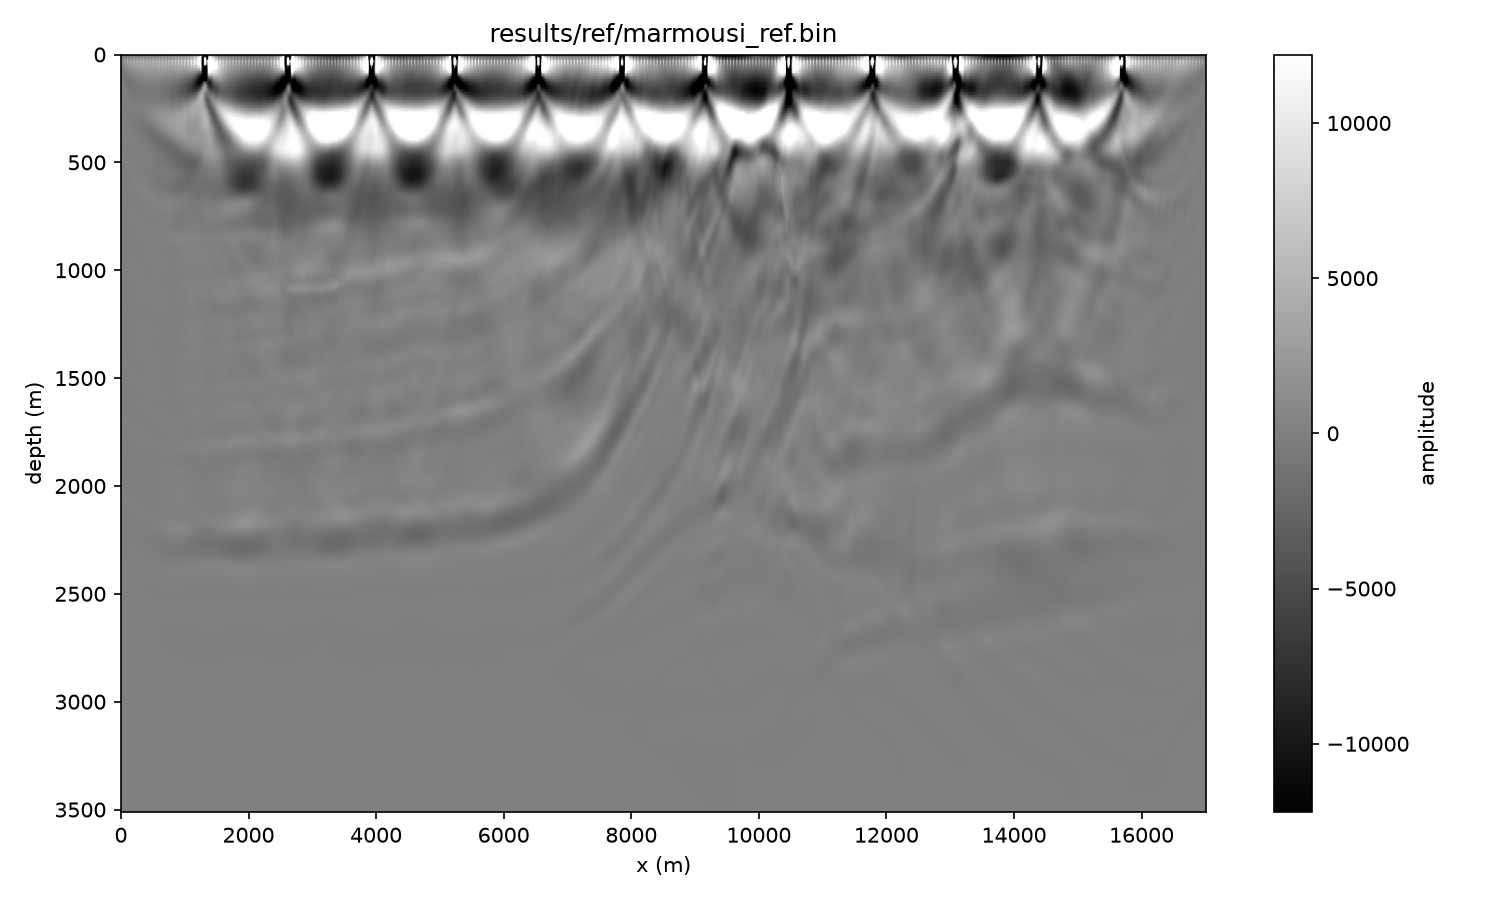
\includegraphics[width=0.85\linewidth]{figures/image_raw.png}\\[4pt]
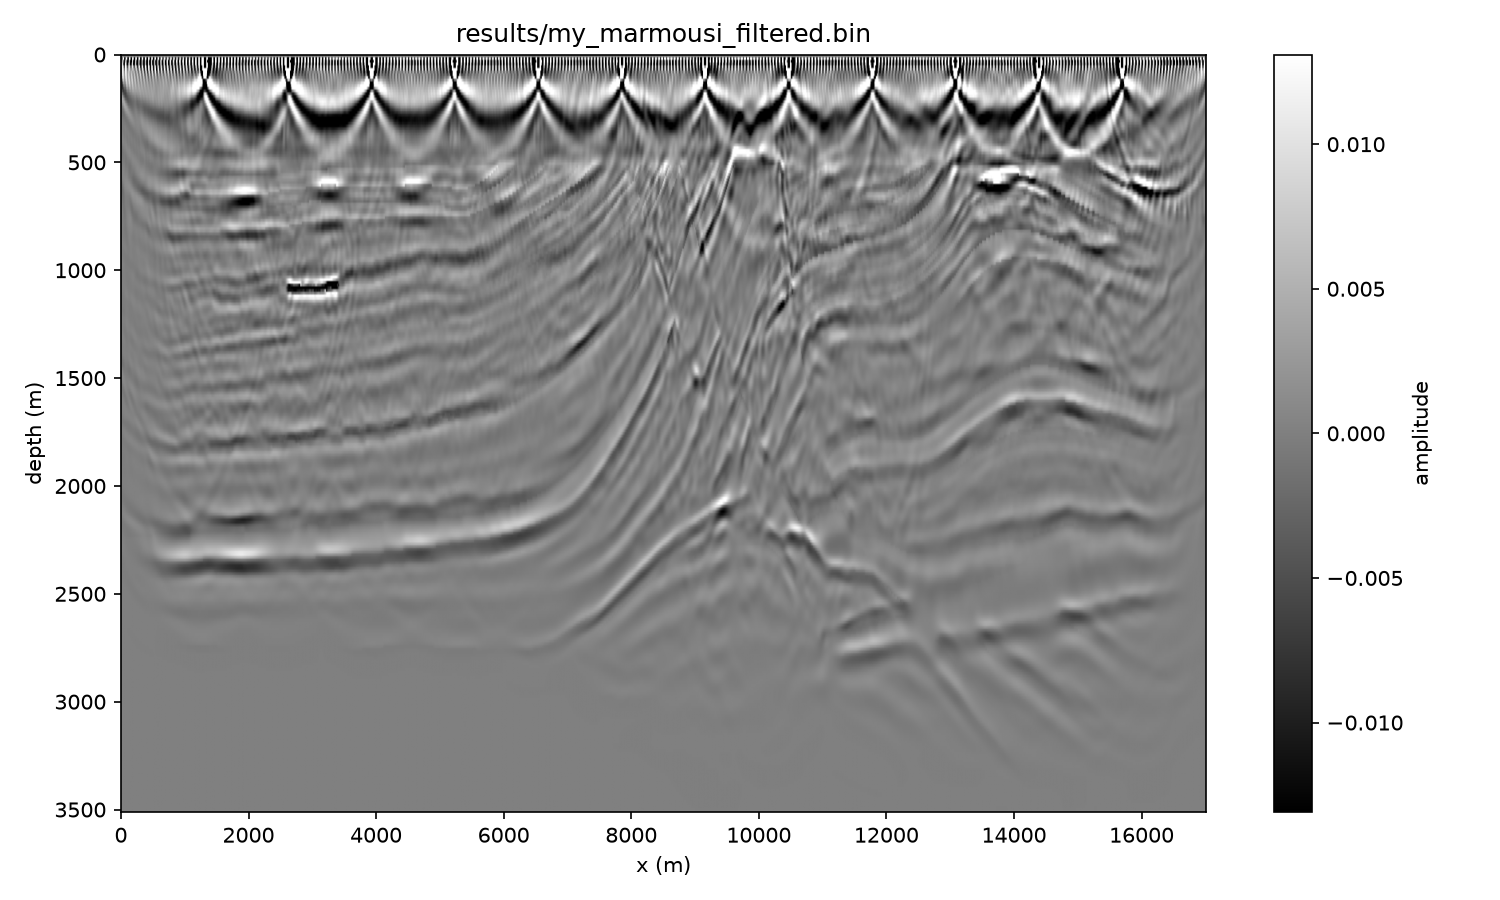
\includegraphics[width=0.85\linewidth]{figures/image_final.png}
\caption{Migrated Marmousi2 section (12 shots, $\Delta x = 12.5$~m).
Top: raw cross-correlation image. Bottom: after illumination compensation
and Laplacian filtering.}
\label{fig:image}
\end{figure}

\paragraph{Every version produces the same image.}
Figure~\ref{fig:versions-grid} shows the image of the CPU reference next to
the images of the five GPU versions, displayed identically. They cannot be
told apart, and the correlation of each GPU image with the reference rounds
to $1.0000000$. Table~\ref{tab:correctness} quantifies the differences on two
GPUs of different generations.

\begin{figure}[H]
\centering
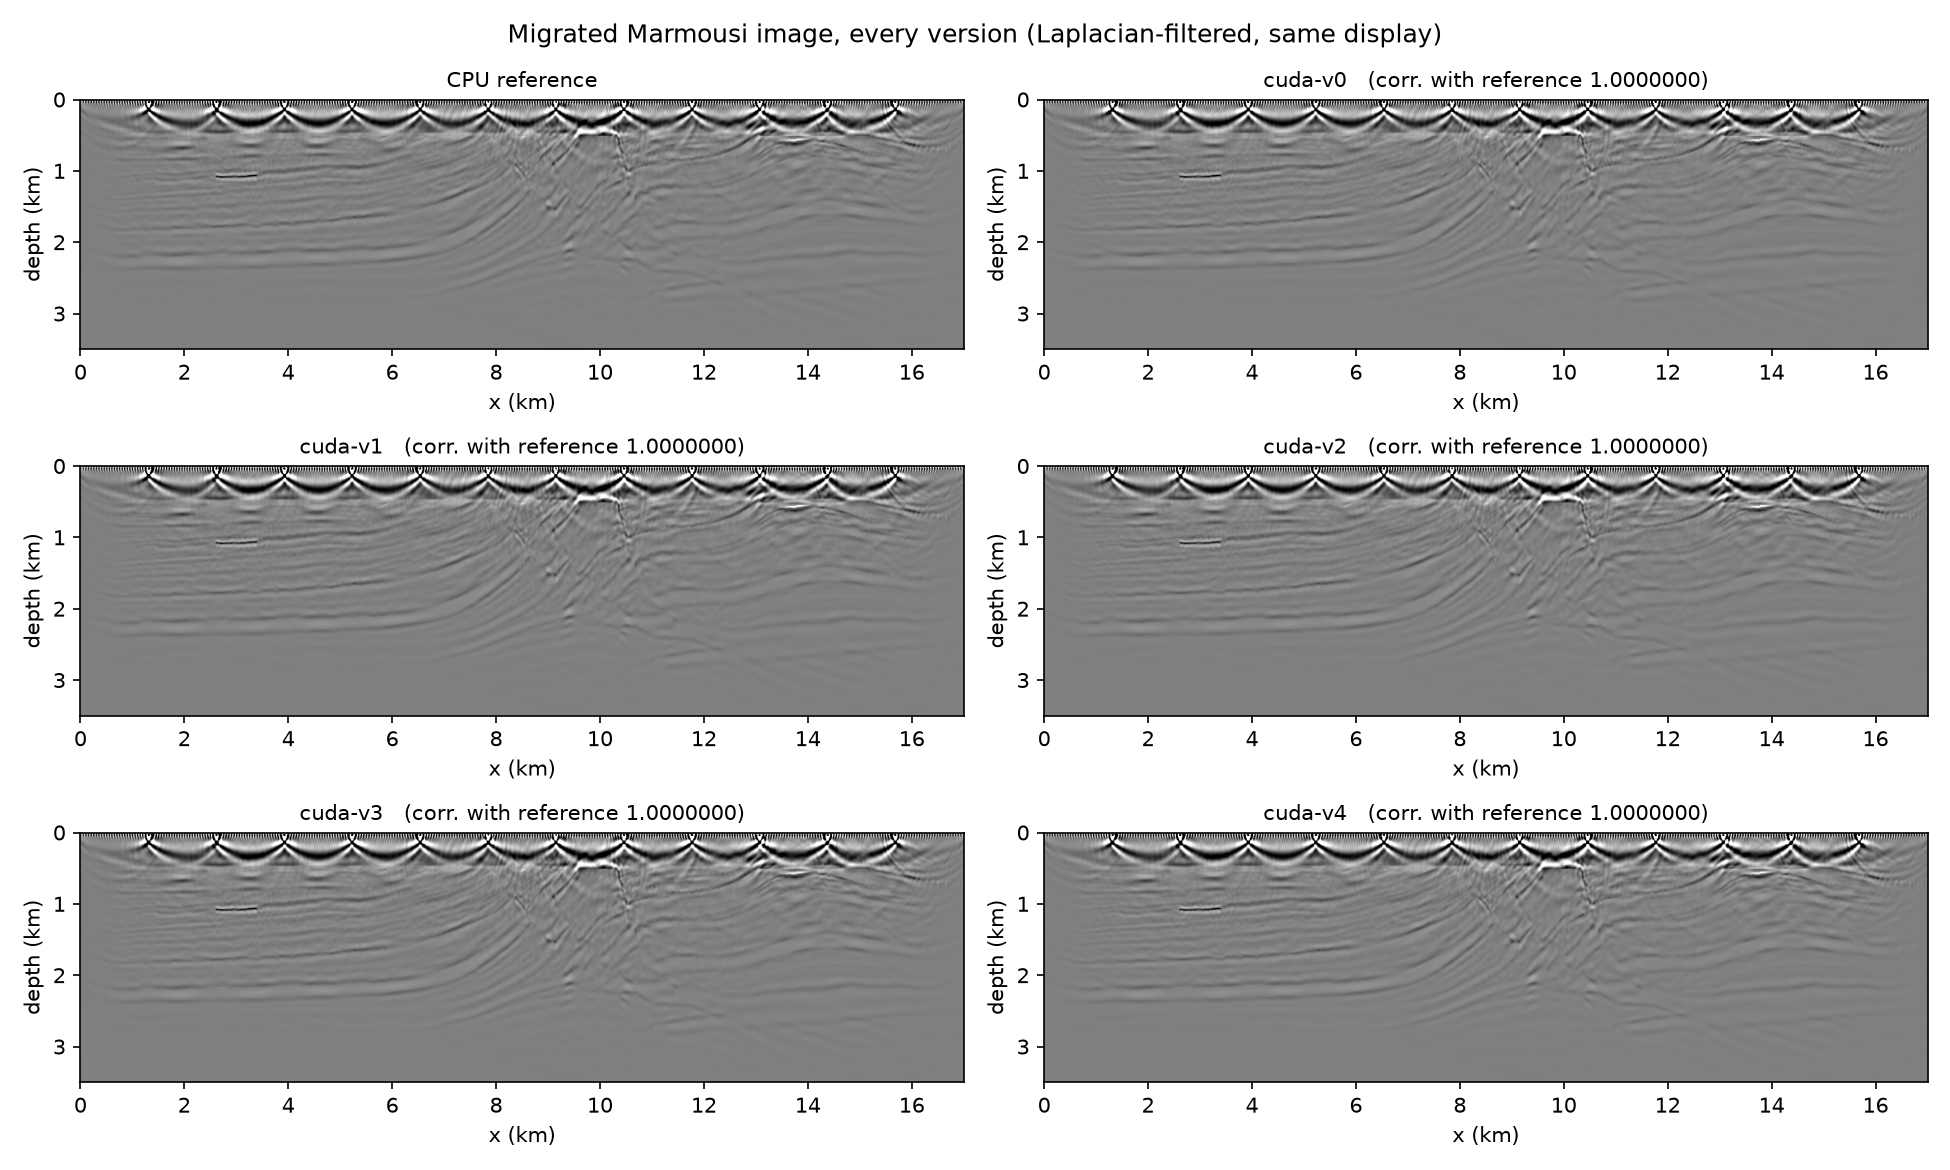
\includegraphics[width=\linewidth]{figures/versions_grid.png}
\caption{The migrated image of the CPU reference and of the five GPU versions
(filtered, same display). The correlation of each GPU image with the
reference is given in its title.}
\label{fig:versions-grid}
\end{figure}

\begin{table}[H]
\centering
\caption{Difference between each engine's image and the CPU reference image:
relative $L_2$ norm of the difference, and correlation.}
\label{tab:correctness}
\begin{tabular}{lccc}
\toprule
       & \multicolumn{2}{c}{Relative $L_2$ difference} & \\
\cmidrule(lr){2-3}
Engine & A40 (Ampere) & RTX PRO 6000 (Blackwell) & Correlation \\
\midrule
Optimized CPU & 0 (bit-identical) & ---                  & 1 \\
v0            & $4.3\times10^{-6}$ & $4.3\times10^{-6}$  & 1.0000000 \\
v1            & $4.2\times10^{-6}$ & $7.3\times10^{-6}$  & 1.0000000 \\
v2            & $4.6\times10^{-6}$ & $7.5\times10^{-6}$  & 1.0000000 \\
v3            & $8.5\times10^{-6}$ & $1.45\times10^{-5}$ & 1.0000000 \\
v4            & $6.7\times10^{-6}$ & $1.06\times10^{-5}$ & 1.0000000 \\
\bottomrule
\end{tabular}
\end{table}

The optimized CPU engine performs exactly the same floating-point operations
as the reference, in the same order, and its image is bit-identical. The
reference itself is reproducible across machines: runs on an AMD and on an
Intel processor gave bit-identical images. The GPU images differ from the
reference by a relative $L_2$ norm of about $10^{-5}$. This is the expected
signature of floating-point rounding: the GPU compiler contracts a
multiplication and an addition into a single fused multiply-add, which rounds
once instead of twice, and small rounding differences accumulate over the
$67\,200$ time steps of the benchmark. A programming error, such as a wrong
index or a missing boundary, produces differences of $10^{-3}$ or more, a
hundred times larger. The differences also depend slightly on the GPU: on the
Blackwell GPU, v3 and v4 land just above the $10^{-5}$ threshold of our
correctness criterion, while their correlation is still exactly 1.
Figure~\ref{fig:version-diff} shows where these differences are: the largest
is $0.53\times10^{-5}$ of the image's peak value, concentrated near the
shallow sources, with no structure resembling a reflector.

\begin{figure}[H]
\centering
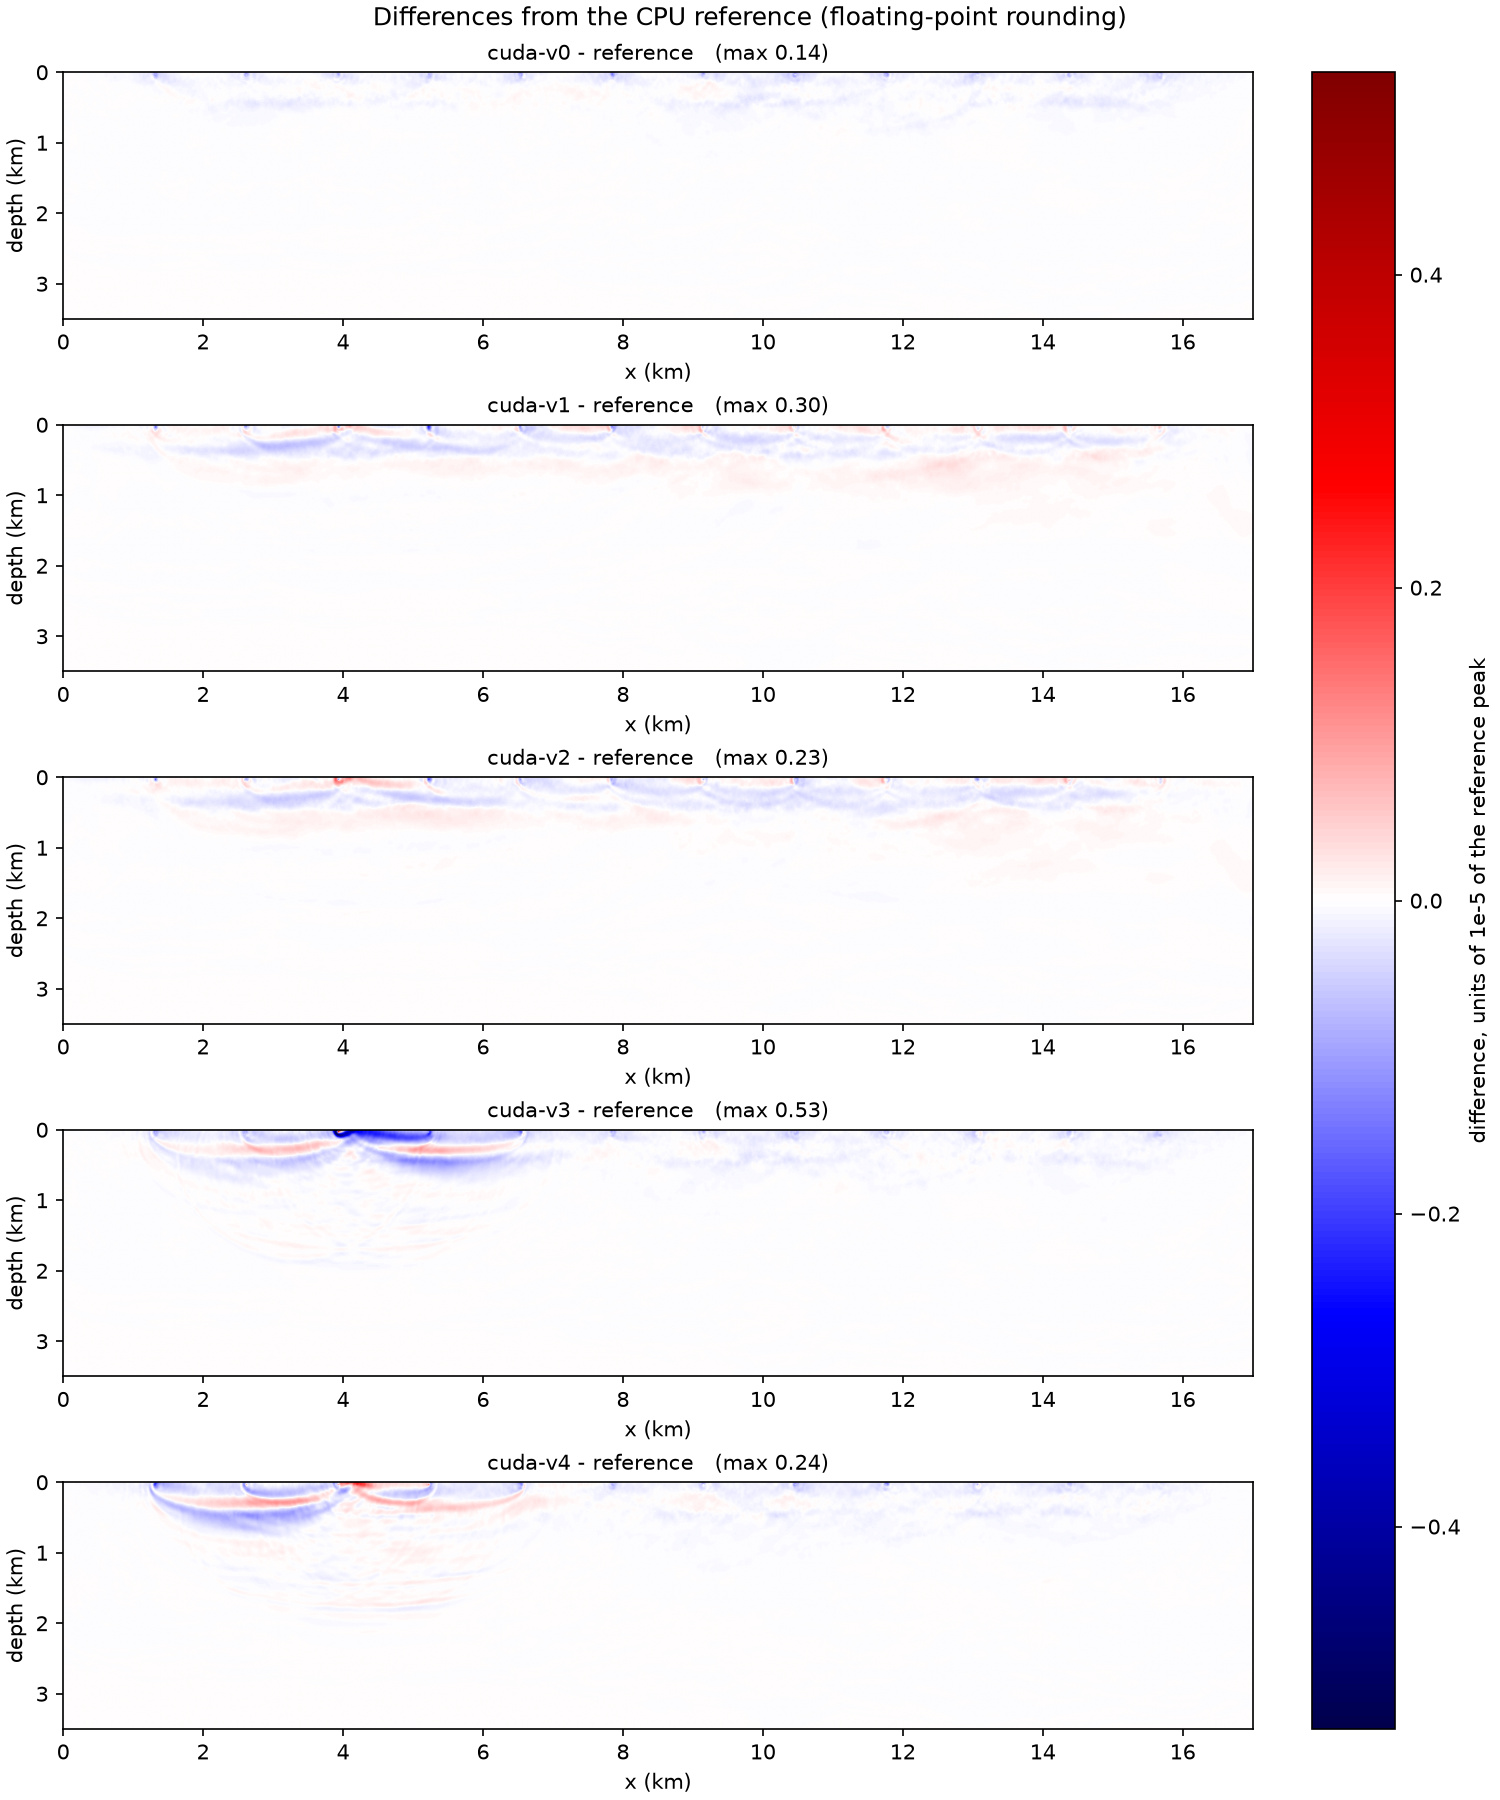
\includegraphics[width=0.8\linewidth]{figures/version_differences.png}
\caption{Difference between each GPU image and the CPU reference, in units of
$10^{-5}$ of the reference's peak value (one color scale for all panels).}
\label{fig:version-diff}
\end{figure}

\paragraph{Comparison with Devito.}
Figure~\ref{fig:devito-image} compares our image with the image computed by
Devito on the same data. The two images show the same geology, with the same
reflectors at the same positions. Their correlation is $0.95$ after the
display filter, and $0.69$ on the raw images. The raw correlation is lower
because the two codes scale the amplitudes differently, and the raw images are
dominated by the low-frequency artefacts, where this difference weighs most.
The visible differences, in particular a stronger horizontal event near
0.4~km depth in Devito's image, come from independent implementation choices:
the absorbing boundary, and the way sources are placed between grid points
(Devito interpolates, our engine uses the nearest grid point). Agreement
between two independently developed codes on the positions of all the
reflectors confirms that our reference solves the intended problem.

\begin{figure}[H]
\centering
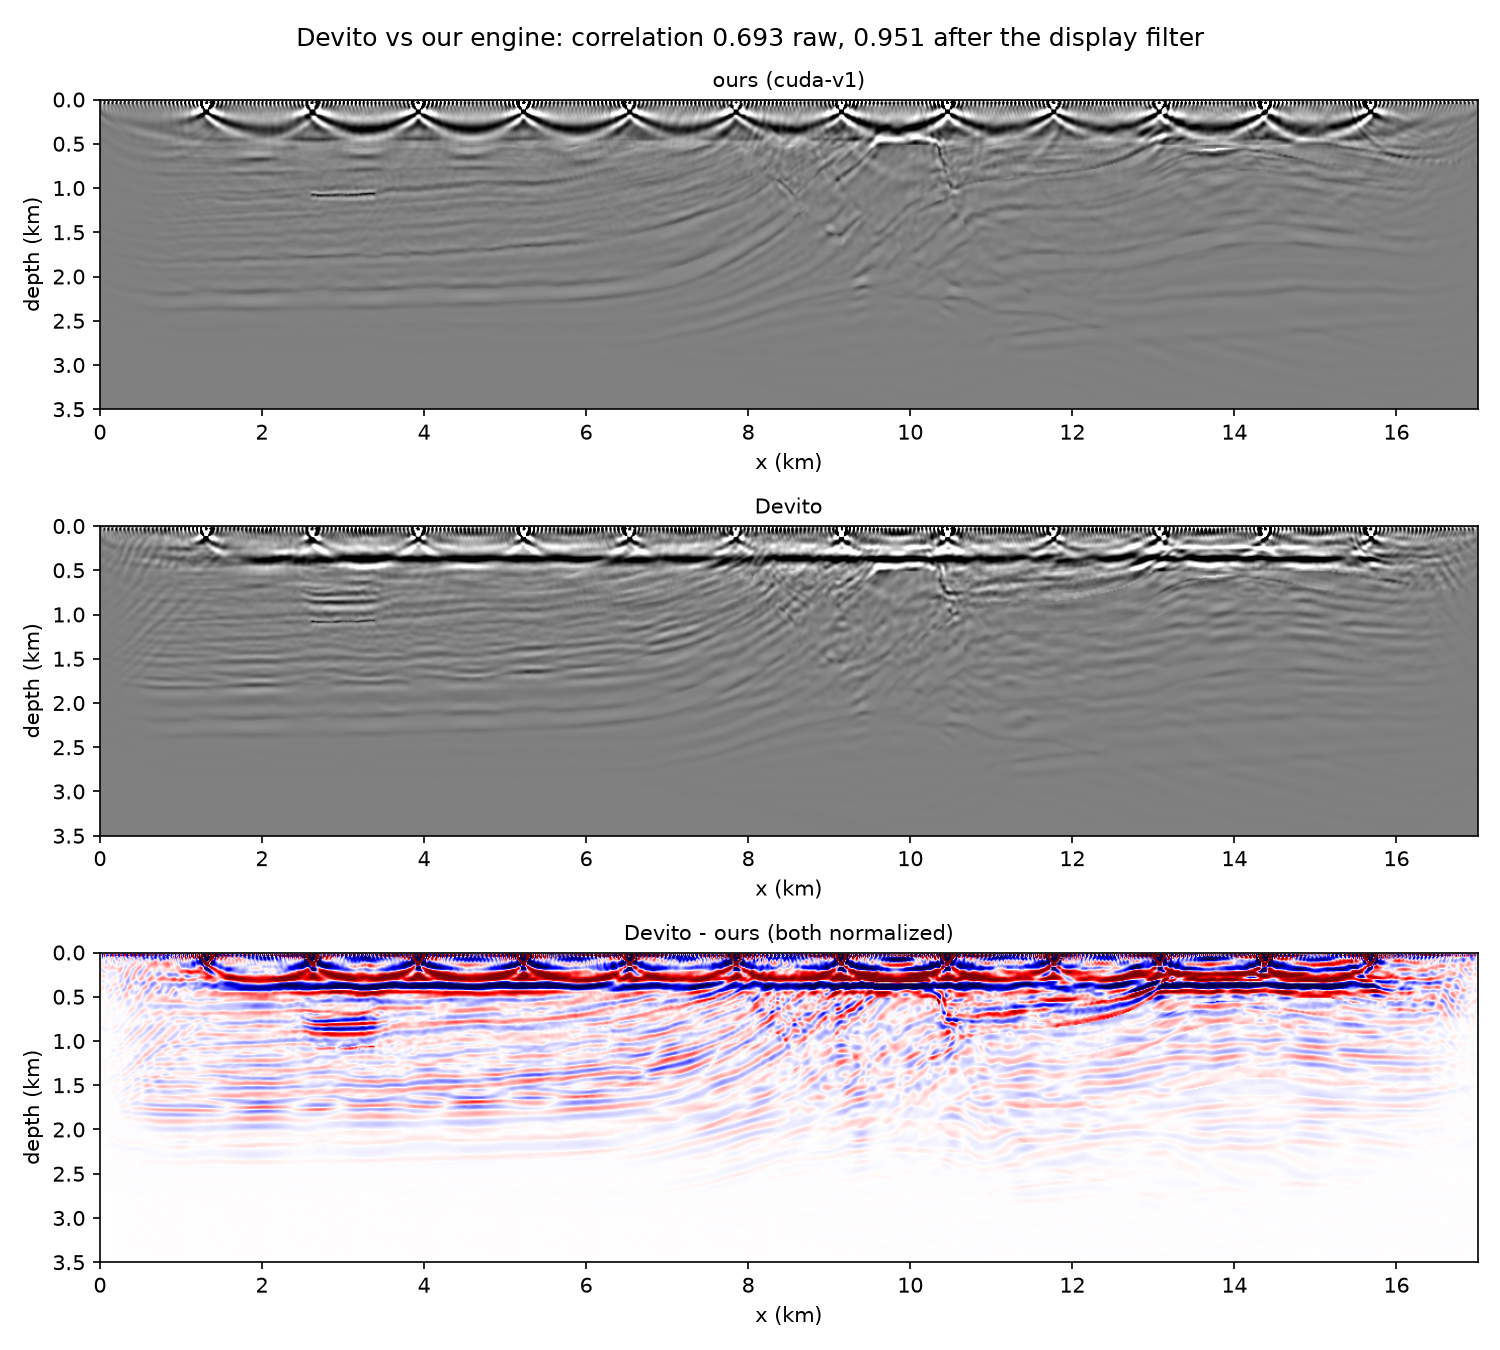
\includegraphics[width=0.8\linewidth]{figures/devito_vs_ours.png}
\caption{Our image (v1, top), Devito's image (middle), and their difference
after normalization (bottom), on the same data.}
\label{fig:devito-image}
\end{figure}

% ---------------------------------------------------------------------------
\subsection{Speed-up over the CPU}

Table~\ref{tab:speedup} and Figure~\ref{fig:time-per-shot} give the time needed
by each engine to migrate the 12 shots. The time is measured from the first
to the last shot, including all data transfers; the reading of the input files
and, for Devito, the compilation of the generated code are excluded.

\begin{table}[H]
\centering
\caption{Time to migrate the 12-shot Marmousi dataset, throughput, and
speed-up relative to the two CPU engines (Xeon Gold 6342, 8 cores; NVIDIA A40).}
\label{tab:speedup}
\begin{tabular}{lrrrrr}
\toprule
       &           &          & Throughput & \multicolumn{2}{c}{Speed-up vs} \\
\cmidrule(lr){5-6}
Engine & Total (s) & Shot (s) & (Gpts/s)   & CPU ref. & opt.\ CPU \\
\midrule
CPU ref.\ (1 core)       & 1016.5 & 84.7   & 0.037 & 1         & ---  \\
Opt.\ CPU (8 cores)      & 498.9  & 41.6   & 0.075 & 2.0       & 1    \\
Devito (GPU)             & 10.2   & 0.853  & 3.7   & 99        & 49   \\
Ours, v0                 & 2.32   & 0.193  & 16.2  & 439       & 215  \\
Ours, v1                 & 2.13   & 0.178  & 20.0  & 476       & 234  \\
Ours, v2                 & 1.88   & 0.156  & 20.0  & 542       & 266  \\
Ours, v3                 & 1.95   & 0.162  & 19.3  & 523       & 256  \\
Ours, v4                 & 1.97   & 0.164  & 19.0  & 516       & 253  \\
\bottomrule
\end{tabular}
\end{table}

\begin{figure}[H]
\centering
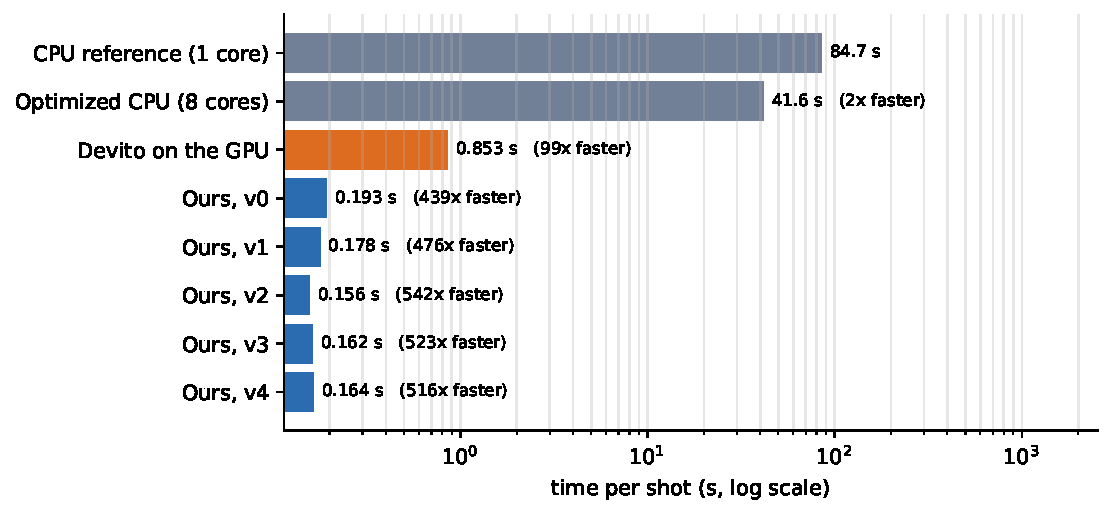
\includegraphics[width=0.9\linewidth]{figures/time_per_shot.pdf}
\caption{End-to-end time per shot of every engine (logarithmic scale), with the
speed-up relative to the CPU reference. For the comparison of the GPU kernels
alone, see Section~\ref{s:devito}.}
\label{fig:time-per-shot}
\end{figure}

\paragraph{The GPU engines are two orders of magnitude faster.}
A shot that takes 84.7~s on one CPU core, and 41.6~s with the optimized code
on 8 cores, takes 0.16 to 0.19~s with our GPU versions: a speed-up of
\textbf{440 to 540} over the reference and \textbf{215 to 266} over the
optimized CPU engine. Devito, running on the same GPU, migrates a shot in
0.85~s: \textbf{99 times} faster than the reference and \textbf{49 times}
faster than the optimized CPU engine. Both GPU implementations are thus far
beyond what the CPU achieves on this platform.

\paragraph{Reading the table correctly.}
Three remarks are needed to interpret these numbers honestly.
\begin{itemize}
\item \emph{The CPU baseline.} The optimized CPU engine is only twice as fast
as the single-core reference. It uses the 8 cores allocated to the cloud
instance; a dedicated multi-socket server would be several times faster, and
the speed-ups over the CPU should be read as ``one A40 compared with this
8-core instance''. The comparison between the GPU engines, all measured on the
same GPU, does not depend on this.
\item \emph{v1 and v2.} v2 appears 13\,\% faster than v1 in the total time.
The propagation itself takes the same time in both (1.87~s); the difference
comes from a one-time operation of v1 outside the kernels, before the first
shot. The per-kernel profile of Section~\ref{s:profile} gives the reliable
comparison.
\item \emph{Devito.} These are end-to-end times. Measured alone, Devito's
stencil kernel is in fact \emph{faster} than ours; Devito loses the end-to-end
comparison because of the time spent moving its saved wavefield between the host
and the GPU. Section~\ref{s:devito} analyses this in detail.
\end{itemize}

% ---------------------------------------------------------------------------
\subsection{Where the GPU time goes}\label{s:profile}

Nsight Systems records every kernel executed by the GPU. Dividing the total
time of each kernel by the $67\,200$ time steps of the benchmark gives the cost
of one time step, broken down by operation (Figure~\ref{fig:step-breakdown}).

\begin{figure}[H]
\centering
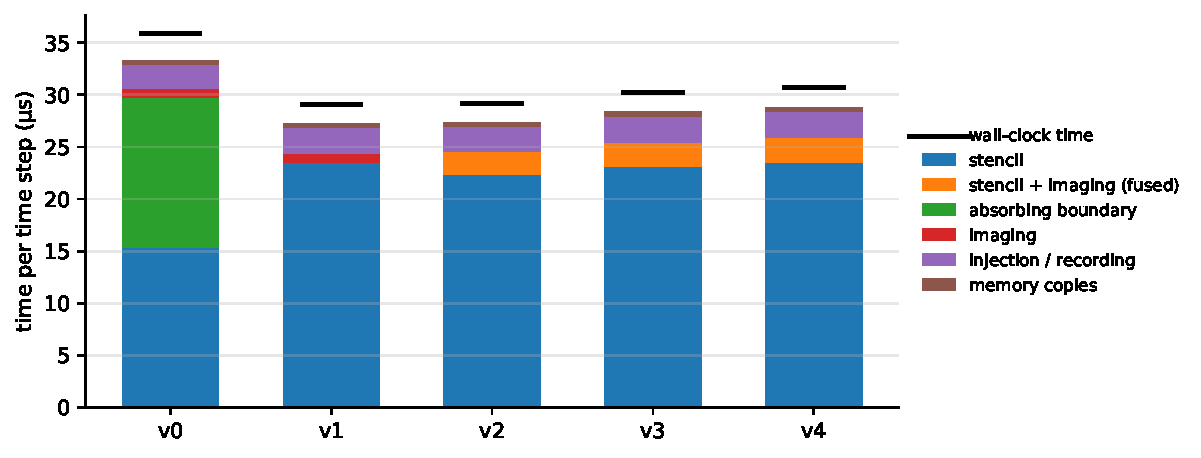
\includegraphics[width=0.9\linewidth]{figures/step_breakdown.pdf}
\caption{GPU time of one time step for each version, broken down by kernel
(Nsight Systems, NVIDIA A40). The black marks give the wall-clock time per
step.}
\label{fig:step-breakdown}
\end{figure}

\paragraph{Merging kernels is the decisive optimization.}
In v0, the stencil takes 15.4~\textmu s per step and the separate
absorbing-boundary kernel 14.4~\textmu s: this second pass over the grid costs
almost as much as the stencil itself, although it performs one multiplication
per point. The reason is that both kernels are limited by memory traffic, not
by computation, and each one reads and writes the whole grid. Merging the two
(v1) removes one full pass: the merged kernel takes 23.5~\textmu s instead of
$15.4 + 14.4 = 29.8$~\textmu s, and the GPU time per step drops from 33.3 to
27.2~\textmu s ($-18\,\%$).

\paragraph{The kernel runs close to the memory bandwidth.}
At 20.0~billion updates per second and 24~bytes per update, v1 moves about
480~GB/s, which is $83\,\%$ of the 578~GB/s we measured on this GPU. The
kernel therefore spends its time waiting for memory, as predicted by the
arithmetic-intensity analysis of Section~\ref{s:computation bottleneck}. This
explains why v3 (shared memory) and v4 (warp shuffles) bring no improvement:
they reduce the number of times a neighbouring value is read, but these
repeated reads were already served by the GPU caches and did not reach the
main memory. They add instructions and synchronization without reducing the
traffic that limits the kernel, and the time per step increases slightly
(28.4 and 28.8~\textmu s).

\paragraph{The CPU barely keeps up.}
The CPU spends about 22~\textmu s per time step launching kernels, while the
GPU needs about 27~\textmu s to execute them. The GPU is busy $93$ to $94\,\%$
of the time; the rest is idle time between kernels. At this grid size, the
cost of launching kernels is almost as large as the work itself, a limit that
disappears on larger grids (next subsection).

% ---------------------------------------------------------------------------
\section{Scaling the workload}\label{s:scaling-section}

The Marmousi dataset used so far is small by industrial standards: 0.56 million
grid points, and a shot migrated in 0.16~s on the GPU. At this size, fixed costs
such as kernel launches still matter, and the GPU memory is almost empty. To
find out how the engines behave on realistic problem sizes, and where their
limits are, we increased the workload in a controlled way and repeated the
measurements with our engine and with Devito.

% ---------------------------------------------------------------------------
\subsection{How the workload was increased}

\paragraph{A finer grid, a higher frequency.}
The workload was increased the way it grows in production: by refining the
grid to image higher frequencies, and therefore finer details. The same
Marmousi2 model was resampled from its original 1.25~m grid with six spacings,
from 12.5~m down to 1.25~m. Three parameters follow from the grid spacing
$\Delta x$:
\begin{itemize}
\item \emph{The source frequency} is raised in proportion,
  $f_0 = 10~\text{Hz} \times 12.5~\text{m}/\Delta x$. A finer grid is only
  useful if the waves it carries are shorter; scaling $f_0$ keeps the number of
  grid points per wavelength constant, so that every grid computes the wave
  with the same accuracy and the comparison between sizes is fair.
\item \emph{The time step} is reduced in proportion,
  $\Delta t = 1~\text{ms} \times \Delta x/12.5~\text{m}$, to respect the
  stability condition of the explicit scheme, which requires
  $\Delta t \propto \Delta x$.
\item \emph{The number of time steps} grows accordingly, $n_t = 2.8~\text{s}/\Delta t$,
  so that every dataset records the same 2.8~s.
\end{itemize}
The absorbing boundary keeps its width of 50 cells: since the wavelength shrinks
with the grid, 50 cells always represent the same number of wavelengths.
Table~\ref{tab:workload} lists the resulting datasets. Each halving of $\Delta x$
multiplies the number of points by 4 and the number of time steps by 2: the work
per shot grows by a factor of 8, and the finest grid represents about 700 times
the work of the original one.

\begin{table}[H]
\centering
\caption{The scaled datasets. Work: grid-point updates per shot (forward and
backward propagation). Memory: snapshots, one every 10 time steps.}
\label{tab:workload}
\begin{tabular}{rrrrrrrr}
\toprule
$\Delta x$ (m) & $f_0$ (Hz) & $\Delta t$ (ms) & $n_t$ & Grid points & Work/shot & $\times$ work & Memory \\
\midrule
12.5 & 10   & 1.0 & 2\,800  & 0.38 M & $3.1\times10^{9}$  & 1   & 0.4 GiB \\
6.25 & 20   & 0.5 & 5\,600  & 1.5 M  & $2.1\times10^{10}$ & 7   & 3.2 GiB \\
5    & 25   & 0.4 & 7\,000  & 2.4 M  & $3.9\times10^{10}$ & 13  & 6.2 GiB \\
3.75 & 33.3 & 0.3 & 9\,334  & 4.2 M  & $8.9\times10^{10}$ & 29  & 14.7 GiB \\
2.5  & 50   & 0.2 & 14\,000 & 9.5 M  & $2.9\times10^{11}$ & 93  & 49.7 GiB \\
1.25 & 100  & 0.1 & 28\,000 & 38 M   & $2.2\times10^{12}$ & 714 & 397 GiB \\
\bottomrule
\end{tabular}
\end{table}

\paragraph{Data generation.}
For each grid, the shot records were computed by our GPU engine (v1), with the
same forward propagator as the migration. On the CPU, modelling a single shot at
1.25~m would take several hours; on the GPU it takes about a minute. Each scaled
dataset contains two shots. The time per shot does not depend on the number of
shots, since shots are migrated one after the other with the same buffers; we
verified this at 12.5~m, where the propagation takes 0.156~s per shot with
the 12-shot dataset and 0.155~s per shot with the 2-shot dataset.

\paragraph{Snapshot interval.}
The source wavefield is saved every 10 time steps on every grid. The interval
is kept constant in \emph{time steps}, not in milliseconds, because the period
of the highest frequency shrinks with $\Delta t$. A first campaign used a fixed
interval of 10~ms, which is adequate at 12.5~m but samples the wavefields too
coarsely at fine grids: at 2.5~m, images computed with snapshots every 5~ms and
every 10~ms correlated at only $0.36$, the signature of aliasing. The interval
was corrected and the memory measurements repeated; the throughput
measurements of that first campaign remain valid, since the snapshot interval
has almost no effect on speed.

\paragraph{The measurement campaign.}
All runs were performed on the A40 platform of Table~\ref{tab:hardware}, by
scripts that run every point automatically:
\begin{itemize}
\item \emph{Grid sweep:} each dataset is migrated with our versions v1 and v3,
  and with Devito on the GPU. For each run we record the time per shot, the
  throughput, the peak GPU memory and the power drawn by the GPU. A run that
  exceeds the available memory is recorded as such and the sweep continues:
  the failure is itself a measurement.
\item \emph{Snapshot sweep:} at 3.75, 2.5 and 1.25~m, the migration is repeated
  with snapshots every 20, 40, 80 and 160 steps, to measure how far the memory
  limit moves and what it costs in image quality.
\item \emph{Order sweep:} at 2.5~m, the stencil order is varied from 4 to 16,
  which increases the arithmetic work per point without changing the grid.
\end{itemize}
Devito reads exactly the same files, with the same parameters, so that every
point of the comparison involves the same computation.

% ---------------------------------------------------------------------------
\subsection{Throughput as the grid grows}\label{s:scaling}

Table~\ref{tab:scaling} and Figure~\ref{fig:throughput-size} give the time per
shot and the throughput of the two codes on each grid.

\begin{table}[H]
\centering
\caption{Time per shot and throughput on the scaled datasets (NVIDIA A40).
OOM: the run exceeded the available memory.}
\label{tab:scaling}
\begin{tabular}{rrrrrr}
\toprule
       & \multicolumn{2}{c}{Ours, v1} & \multicolumn{2}{c}{Devito (GPU)} & \\
\cmidrule(lr){2-3}\cmidrule(lr){4-5}
$\Delta x$ (m) & s/shot & Gpts/s & s/shot & Gpts/s & Ours vs Devito \\
\midrule
12.5 & 0.156 & 20.1 & 0.853 & 3.7 & 5.5$\times$ \\
6.25 & 0.994 & 21.1 & 3.59  & 5.8 & 3.6$\times$ \\
5    & 1.83  & 21.6 & 6.61  & 5.9 & 3.6$\times$ \\
3.75 & 4.08  & 22.1 & 12.7  & 7.0 & 3.1$\times$ \\
2.5  & 13.0  & 22.4 & OOM   & --- & --- \\
1.25 & 97.9  & 22.8 & OOM   & --- & --- \\
\bottomrule
\end{tabular}
\end{table}

\begin{figure}[H]
\centering
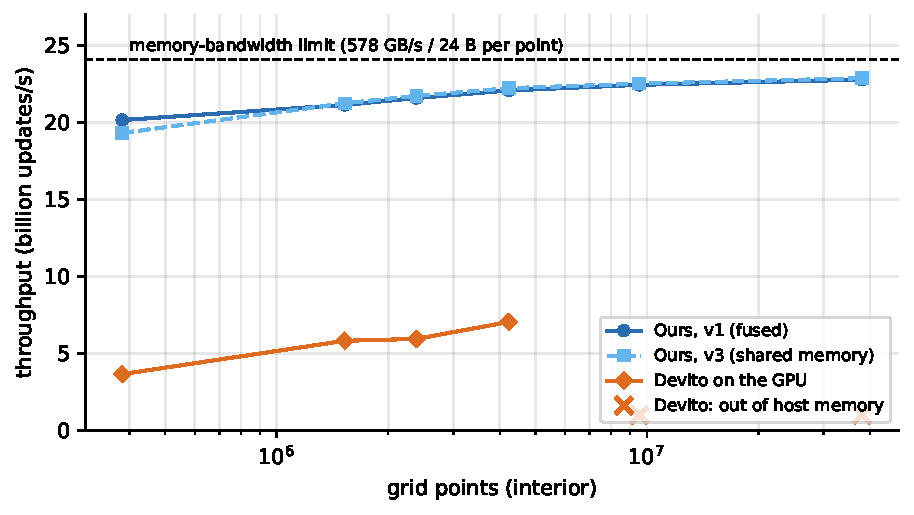
\includegraphics[width=0.9\linewidth]{figures/throughput_vs_size.pdf}
\caption{Throughput as a function of the number of grid points (NVIDIA A40).
The dashed line is the limit set by the measured memory bandwidth.}
\label{fig:throughput-size}
\end{figure}

\paragraph{Our engine reaches the bandwidth limit.}
As the work per shot grows by a factor of 700, the time per shot of our engine
grows by a factor of 630: the throughput \emph{increases}, from 20.1 to
22.8~billion updates per second. On larger grids, each kernel runs longer, and
the fixed cost of launching it, which was almost as large as the work at
12.5~m (Section~\ref{s:profile}), becomes negligible. At 22.8~billion updates per
second and 24~bytes per update, the kernel moves about 550~GB/s, $95\,\%$ of the
578~GB/s measured on this GPU (dashed line). No further gain is possible
without reducing the number of bytes moved per point. A shot at 1.25~m, which
would take about 17~hours on one CPU core, takes 98~seconds.

\paragraph{Shared memory does not help, even on large grids.}
v3 runs at the same speed as v1 on every grid (19.3 to 22.9~billion updates per
second), including at 38~million points, a grid far larger than the 6~MB cache
of the GPU. The reuse of neighbouring values that shared memory is designed to
provide is already obtained from the caches, and the kernel remains limited by
the memory bandwidth, not by repeated reads.

\paragraph{Devito improves with size, but stays three times slower.}
Devito's throughput doubles between the smallest and the largest grid it could
process (3.7 to 7.0~billion updates per second), a sign that part of its time is
a fixed cost per shot that larger problems amortize. It remains three to five
times slower than our engine end to end, although its stencil kernel alone is
faster than ours (Section~\ref{s:devito}): most of its time is spent moving the
saved wavefield, which Devito keeps in the \emph{host} memory and copies between
the host and the GPU. Two observations confirm it. When
snapshots are saved four times less often (Figure~\ref{fig:throughput-order}),
Devito's throughput more than doubles, to 16~billion updates per second. And
at 2.5 and 1.25~m, the operating system stopped Devito for exceeding the 50~GB
of host memory of the instance, while the GPU memory was not full.

% ---------------------------------------------------------------------------
\subsection{Increasing the work per point: the stencil order}

Raising the stencil order from 4 to 16 multiplies the number of floating-point
operations per point by about four, on the same grid ($\Delta x = 2.5$~m,
snapshots every 40 steps). Figure~\ref{fig:throughput-order} shows the effect.

\begin{figure}[H]
\centering
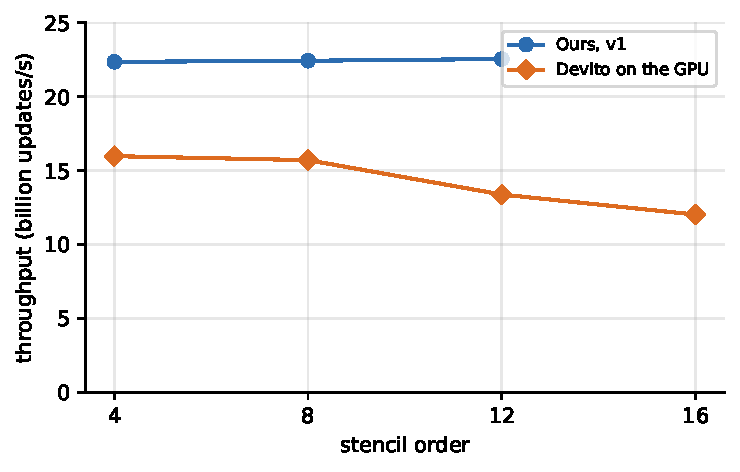
\includegraphics[width=0.7\linewidth]{figures/throughput_vs_order.pdf}
\caption{Throughput as a function of the order of the finite-difference
stencil ($\Delta x = 2.5$~m, NVIDIA A40).}
\label{fig:throughput-order}
\end{figure}

The throughput of our engine does not change: 22.4, 22.4 and 22.6~billion
updates per second at orders 4, 8 and 12. Tripling the arithmetic costs nothing,
because the arithmetic units spend most of their time waiting for memory and
absorb the extra operations for free. This is the most direct experimental
signature of a memory-bound kernel. Devito slows down at high orders, from 16.0
to 12.0~billion updates per second between orders 4 and 16.

% ---------------------------------------------------------------------------
\subsection{The memory limit}

Speed is not the only limit: the saved source wavefield must fit in the GPU
memory. Figure~\ref{fig:capacity} shows the memory used by our engine as a
function of the grid size, for several snapshot intervals.

\begin{figure}[H]
\centering
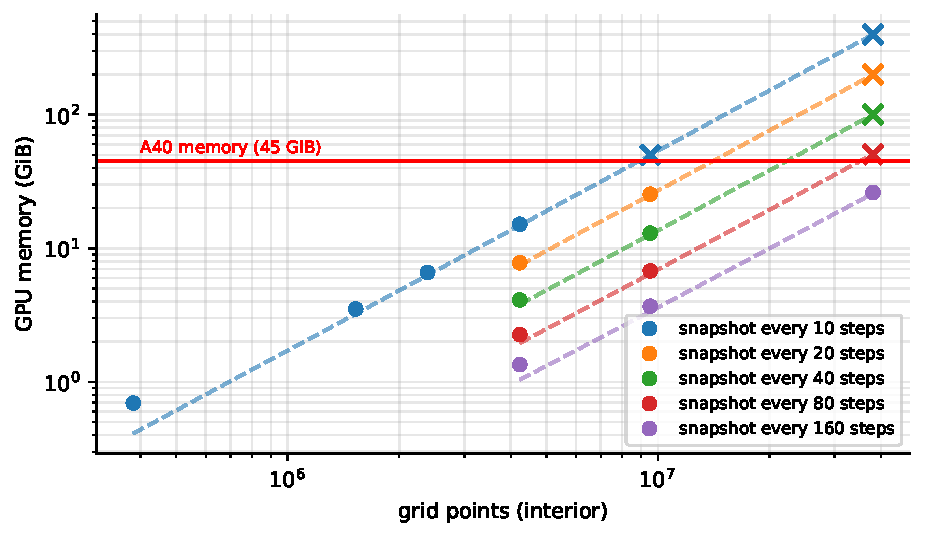
\includegraphics[width=0.9\linewidth]{figures/capacity.pdf}
\caption{GPU memory needed as a function of the grid size, for several snapshot
intervals. Dots: measured. Dashed lines: model. Crosses: runs that exceeded the
memory of the A40 (red line).}
\label{fig:capacity}
\end{figure}

The measured points follow the model of Section~\ref{s:computation bottleneck}:
with a snapshot every 10 time steps, the memory grows as $1/\Delta x^{3}$, from
0.7~GiB at 12.5~m to 15.2~GiB at 3.75~m. At 2.5~m it would need about 50~GiB,
more than the 45~GiB available: this is the limit of one A40. Saving fewer
snapshots moves the limit: at 2.5~m, one snapshot every 20 steps fits in 25~GiB;
at 1.25~m, only one snapshot every 160 steps fits.

\begin{figure}[H]
\centering
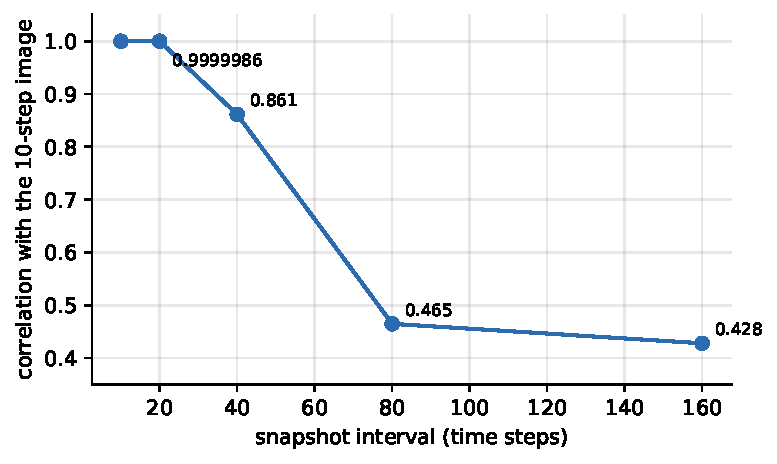
\includegraphics[width=0.7\linewidth]{figures/snapshot_accuracy.pdf}
\caption{Correlation of the image obtained with a larger snapshot interval with
the image obtained with a snapshot every 10 steps ($\Delta x = 3.75$~m).}
\label{fig:snapshot-accuracy}
\end{figure}

Saving fewer snapshots has a price (Figure~\ref{fig:snapshot-accuracy}). The
imaging condition samples the two wavefields at the snapshot times; if the
interval becomes longer than about half the period of the highest frequency
present, the sampling theorem is violated and the image degrades. With one
snapshot every 20 steps, the image is unchanged (correlation $0.9999986$) for
half the memory. With 40 steps the correlation falls to $0.86$, and beyond it the
image is destroyed ($0.47$ and $0.43$). At 1.25~m, a single A40 can therefore only
hold an unusable image: problems of this size require several GPUs, or techniques
that avoid storing the whole wavefield, such as checkpointing or compression.

The two codes hit different limits. Our engine keeps the snapshots in GPU
memory, so its limit is the 45~GiB of the GPU. Devito keeps them in host memory,
so its limit is the RAM of the machine, here 50~GB, and every snapshot crosses
the host--GPU link. On a machine with more RAM, Devito could process grids that
do not fit in the GPU memory, at the cost of these transfers.

% ---------------------------------------------------------------------------
\subsection{Impact on a seismic survey}

To express the measured throughput in terms of production, we project the time
needed to migrate a survey of 1000 shots at $\Delta x = 2.5$~m
(Figure~\ref{fig:survey}). The GPU times are the measured time per shot at this
size, multiplied by the number of shots; since shots are independent, $n$ GPUs
divide the time by $n$. The CPU times are extrapolated from the throughput
measured at 12.5~m.

\begin{figure}[H]
\centering
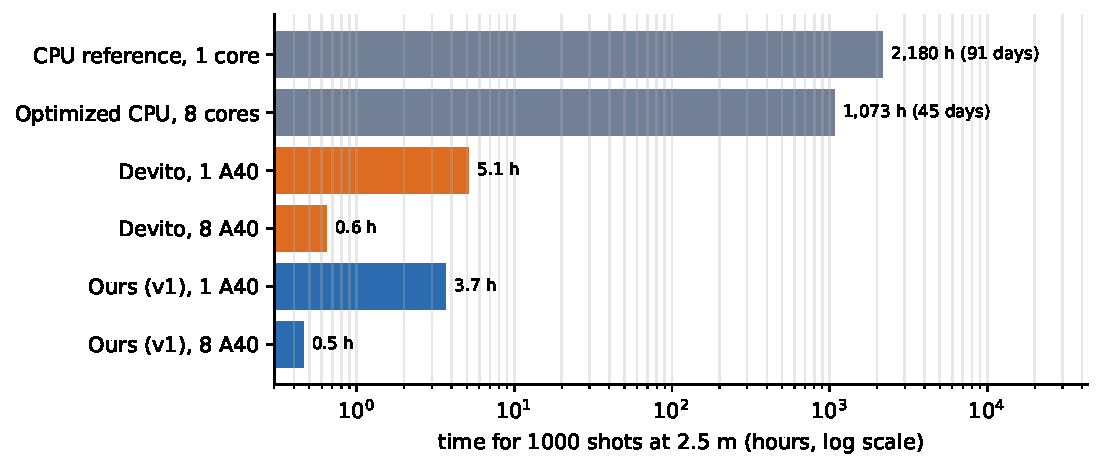
\includegraphics[width=0.9\linewidth]{figures/survey.pdf}
\caption{Projected time to migrate 1000 shots at $\Delta x = 2.5$~m (logarithmic
scale).}
\label{fig:survey}
\end{figure}

On the CPU, the survey would take 2180 hours (91 days) with the reference and
1073 hours (45 days) with the optimized engine. On a single A40 it takes 3.7 hours
with our engine and 5.1 hours with Devito; on 8 GPUs, less than an hour. For a
processing team, this is the difference between a result delivered in weeks and
a result delivered within the working day, which also makes it possible to repeat
the migration several times, for example to test velocity models. These
projections assume that every shot has the same size and that reading the data
is not a bottleneck; they give an order of magnitude, not a production schedule.

\section{Devito versus our engine: faster kernels, slower pipeline}\label{s:devito}

Figure~\ref{fig:time-per-shot} and Table~\ref{tab:scaling} show our engine three
to five times faster than Devito per shot. These are end-to-end times: they
include everything that happens during a shot. Nsight Systems lets us separate
the time spent computing on the GPU from the rest, and this separation reverses
the conclusion: \emph{Devito's stencil kernel is faster than ours}. Devito loses
the end-to-end comparison because of the way it manages the saved wavefield.

% ---------------------------------------------------------------------------
\subsection{Devito's stencil kernel is faster}

Table~\ref{tab:devito-kernels} gives, for each grid, the time of one execution of
the stencil kernel (one time step) and the corresponding throughput, measured by
Nsight Systems on the same A40 and the same data. Devito's kernel is faster on
every grid, by 7\,\% on the smallest and by 23 to 29\,\% from 6.25~m onwards
(Figure~\ref{fig:devito-kernels}a).

\begin{table}[H]
\centering
\caption{Stencil kernel alone (one time step) and complete shot, for our engine
(v1) and Devito, on the A40. Kernel times from Nsight Systems; shot times from the
timed runs. The 2.5~m runs save a snapshot every 40 steps.}
\label{tab:devito-kernels}
\begin{tabular}{rrrrrrr}
\toprule
 & \multicolumn{2}{c}{Kernel time (\textmu s)} & \multicolumn{2}{c}{Kernel (Gpts/s)} & \multicolumn{2}{c}{Shot (s)} \\
\cmidrule(lr){2-3}\cmidrule(lr){4-5}\cmidrule(lr){6-7}
$\Delta x$ (m) & Ours & Devito & Ours & Devito & Ours & Devito \\
\midrule
12.5 & 23.5  & 21.9  & 23.7 & 25.4 & 0.155 & 0.853 \\
6.25 & 82.6  & 66.9  & 22.6 & 27.9 & 1.02  & 3.59  \\
5    & 123.8 & 98.7  & 22.7 & 28.4 & 1.89  & 6.61  \\
3.75 & 209.7 & 165.6 & 22.8 & 28.9 & 4.22  & 12.7  \\
2.5  & 452.1 & 351.3 & 22.9 & 29.5 & 13.0  & 18.5  \\
\bottomrule
\end{tabular}
\end{table}

\paragraph{Why: Devito moves fewer bytes per point.}
Both kernels are limited by memory bandwidth, so the one that moves fewer bytes
per point is faster. The two codes apply the absorbing boundary differently:
\begin{itemize}
\item \emph{Our kernel} reproduces the CPU reference exactly, which damps both
  wavefields at every step. Per point it reads $P$, $P^{\mathrm{prev}}$,
  $(v\Delta t)^2$ and the damping coefficient, and writes both the damped $P$ and
  $P^{\mathrm{next}}$: \textbf{24 bytes}.
\item \emph{Devito's kernel} damps only the new wavefield. It reads the same four
  arrays but writes only $P^{\mathrm{next}}$: \textbf{20 bytes}.
\end{itemize}
The ratio of the traffic, $24/20 = 1.2$, is close to the ratio of the measured
kernel times at 3.75~m, $209.7/165.6 = 1.27$. Both kernels run at the limit of the
memory bandwidth: $22.8 \times 24 \approx 550$~GB/s for ours and
$28.9 \times 20 \approx 580$~GB/s for Devito, against 578~GB/s measured by our
bandwidth test. Devito's compiler also reduces the number of floating-point
operations of the stencil, by factorizing common terms; for a memory-bound kernel
this has no effect on speed.

% ---------------------------------------------------------------------------
\subsection{Devito's pipeline is slower}

Figure~\ref{fig:devito-kernels}b breaks down one complete shot at 3.75~m into the
time the GPU spends computing, transferring data, and waiting.

\begin{figure}[H]
\centering
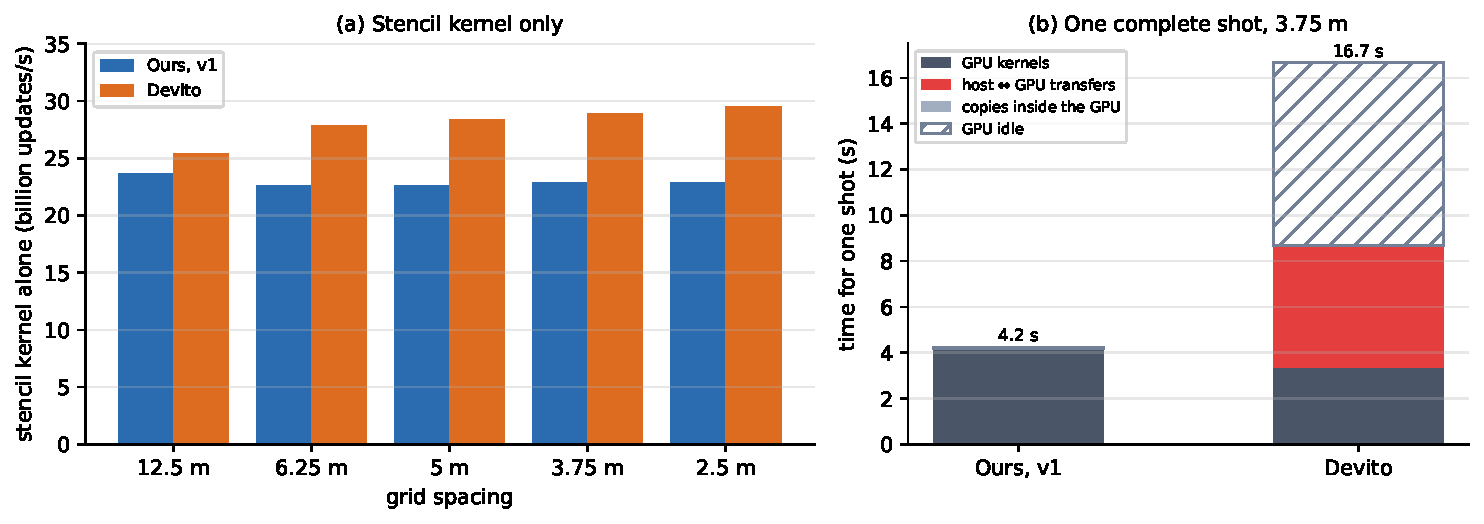
\includegraphics[width=\linewidth]{figures/devito_kernels_vs_end_to_end.pdf}
\caption{(a) Throughput of the stencil kernel alone: Devito is faster on every
grid. (b) One complete shot at 3.75~m, as recorded by Nsight Systems: our GPU
computes almost all the time, while Devito's GPU spends most of the shot
transferring data or idle.}
\label{fig:devito-kernels}
\end{figure}

\paragraph{Our engine: the GPU computes all the time.}
Of the 4.2~s of a shot, 4.1~s are spent in kernels. The snapshots are copied
inside the GPU memory (0.07~s per shot), and almost nothing crosses the link
between the host and the GPU: about 0.05~GB per shot, for the recorded traces and
the final image.

\paragraph{Devito: the saved wavefield crosses the host--GPU link three times.}
In the configuration we used, Devito's default, the saved forward wavefield is
stored in the \emph{host} memory. At 3.75~m this array holds 17.9~GB per shot
(about 930 snapshots of the extended grid). Nsight Systems records 36.7~GB transferred
from the host to the GPU and 18.4~GB from the GPU to the host for one shot:
55~GB, which corresponds to the array crossing the link three times (to the GPU
before the forward propagation, back to the host after it, to the GPU again
before the backward propagation). The link between the host and the GPU (PCIe)
delivers 10 to 12~GB/s in these transfers, about 50 times less than the GPU's own
memory. These transfers take 5.3~s per shot, more than Devito's kernels
(3.4~s).

\paragraph{The rest of the time, the GPU waits.}
The remaining part of Devito's shot is time during which the GPU is idle,
waiting for the host. It includes the work done by the host on the 17.9~GB
array and the preparation of each shot. In the profiled run it also includes the
overhead of Devito's own detailed profiler, which we enabled for this measurement:
this is why the profiled shot lasts 16.7~s, against 12.7~s in the timed run of
Table~\ref{tab:devito-kernels}. The split of this idle time between its causes was
not measured.

\paragraph{Consistent observations.}
This explanation accounts for the other measurements of Section~\ref{s:scaling-section}:
\begin{itemize}
\item the gap between the two codes grows with the number of snapshots, and
  Devito's throughput more than doubles when snapshots are saved four times less
  often;
\item at 2.5 and 1.25~m, Devito was stopped for exceeding the 50~GB of \emph{host}
  memory, while the GPU memory was not full;
\item Devito's GPU draws less power than ours on the same grid (115~W against
  241~W at 3.75~m): it is idle for a larger part of the time.
\end{itemize}

% ---------------------------------------------------------------------------
\subsection{What this comparison teaches}

The two codes are each better at one level, and each points to an improvement of
the other.
\begin{itemize}
\item \emph{Devito's kernel shows the way to a faster kernel for us.} Damping only
  the new wavefield would reduce our traffic from 24 to 20 bytes per point, a gain
  of about 20\,\% on a memory-bound kernel. The price is that the image would no
  longer be bit-identical to our CPU reference, which damps both wavefields; the
  reference would have to be adapted accordingly.
\item \emph{Our pipeline shows the way to a faster Devito.} When the saved
  wavefield fits in the GPU memory, keeping it there removes the transfers and
  most of the idle time. Devito provides options to control where such arrays are
  stored; we used its default configuration, which favors problems larger than
  the GPU memory, at the cost of speed on problems that fit.
\end{itemize}
The end-to-end ranking of Figure~\ref{fig:time-per-shot} therefore reflects data
management choices, not the quality of the generated code: at the level of the
stencil itself, the code generated by Devito outperforms our hand-written kernel.

\section{Conclusion}\label{s:conclusion}

This report studied the acceleration of Reverse Time Migration on GPU
architectures. Starting from a simple and reproducible CPU reference, we built
an optimized CPU engine and five successive GPU versions, validated every one
of them against the reference, profiled them with Nsight Systems, measured
their behavior on problems up to 700 times larger than the original, and
compared them with Devito, an established framework for finite-difference
codes.

\paragraph{Main findings.}
\begin{itemize}
\item \emph{The results are correct.} All GPU versions produce the image of the
  CPU reference to within floating-point rounding (relative difference below
  $1.5\times10^{-5}$ on two GPU generations), and Devito, developed
  independently, images the same reflectors at the same positions.
\item \emph{The GPU changes the scale of the problem.} On one NVIDIA A40, a shot
  is migrated 440 to 540 times faster than with the CPU reference and 215 to 266
  times faster than with the optimized CPU engine on the 8 cores of the cloud
  instance. A survey of 1000 shots at 2.5~m, estimated at 91 days on one CPU
  core, takes 3.7 hours on one GPU.
\item \emph{RTM is limited by memory bandwidth.} The kernels move 83 to 95\,\%
  of the measured bandwidth and use less than 2\,\% of the arithmetic
  capability. This single fact explains every optimization result: merging
  kernels, which removes passes over memory, is the only clear gain ($-18\,\%$
  per time step); shared memory and warp shuffles, which reduce reads already
  served by the caches, bring nothing, even on grids far larger than the cache;
  and raising the stencil order costs no time at all.
\item \emph{Memory, not speed, limits the problem size.} The saved wavefield
  grows as $1/\Delta x^{3}$, and one A40 reaches its limit between 3.75 and
  2.5~m. Saving fewer snapshots helps only up to a point: every 20 steps is
  free, every 40 steps already degrades the image.
\item \emph{Kernels and data management are two separate problems.} Devito's
  generated stencil kernel is 7 to 29\,\% faster than ours, because it moves 20
  instead of 24 bytes per point, yet Devito is three to five times slower end to
  end, because its default configuration keeps the saved wavefield in host
  memory and transfers it over PCIe.
\end{itemize}

\paragraph{Limitations.}
The study has several limits, which bound the scope of its conclusions. The
GPU performance counters were not accessible on the cloud platform, so the
kernel analysis relies on timelines, timings and a model of the memory traffic
rather than on hardware counters. The problem is two-dimensional, acoustic and
of constant density. The shot records are synthetic and were computed by our
own engine, which validates the implementation but not the physical model. All
measurements use a single GPU, the CPU baseline is a small cloud instance, and
Devito was run with its default configuration.

\paragraph{Future work.}
Each result points to a next step:
\begin{itemize}
\item reduce the traffic of our kernel from 24 to 20 bytes per point, as Devito
  does, which should bring about 20\,\% on a memory-bound kernel;
\item reduce the launch overhead measured on small grids, for example with
  CUDA Graphs, which submit a whole sequence of kernels at once;
\item remove the memory limit with checkpointing or wavefield compression, and
  distribute the independent shots over several GPUs;
\item extend the engine to three dimensions, where both the computing and the
  memory requirements grow by another order of magnitude;
\item complete the kernel analysis with Nsight Compute on a machine that
  exposes the GPU counters, and repeat the Devito comparison with the saved
  wavefield kept in GPU memory.
\end{itemize}

More generally, this work shows that the performance of a seismic imaging code
on a GPU depends less on the arithmetic it performs than on the data it moves:
the number of bytes per grid point, and where the saved wavefield lives. These
two quantities, rather than the number of operations, are the ones to optimize.

\bibliography{\bib}

\end{document}
